\documentclass[oneside,11pt]{lib/PhDthesisPSnPDF}

\usepackage[utf8]{inputenc}
\usepackage{epsfig}
\usepackage{amsmath,amssymb,amsfonts,latexsym}
\usepackage{enumerate}
\usepackage{xspace}
\usepackage{epsf,picinpar}
\usepackage{varioref}
\usepackage{colortbl,multirow,hhline}
\usepackage{listings}
\usepackage{amssymb}
\usepackage{colortbl,multirow,hhline}
\usepackage{algorithmic}
\usepackage{algorithm}
\usepackage{caption}
\usepackage[normalem]{ulem}
\usepackage{xcolor}
\usepackage{pifont}
\usepackage{xcolor,colortbl}
\usepackage{url}
\usepackage{balance}
\usepackage{graphicx, subfigure}
\usepackage{longtable}
\usepackage{lscape}
\usepackage{multirow}
\usepackage{listings}
\usepackage{framed}
\usepackage{morefloats}
\usepackage[T1]{fontenc}
\usepackage{array}
\usepackage{pdfpages}
\usepackage{fancybox}
\usepackage{amsmath}
\usepackage{flushend}
\usepackage{booktabs}
\usepackage{enumitem}
\usepackage{pbox}
\usepackage{fancyvrb}
\usepackage{cprotect}
\usepackage{fontspec}
\usepackage{tabularx}

\let\cleardoublepage\clearpage


\textwidth 15cm
\textheight 22cm
\parindent 10pt
\oddsidemargin 0.85cm
\evensidemargin 0.37cm


\makeatletter
\g@addto@macro{\UrlBreaks}{\UrlOrds}
\makeatother

\newcommand{\source}[1]{\caption*{Source: {#1}}}
\newcommand{\limit}[1]{\textcolor{red}{\ding{46}~Page limit:~#1}\\}
\newcommand{\todo}[1]{\textcolor{blue}{\ding{46}~#1}} 
\newcommand{\ie}{\emph{i.e.,}\xspace}
\newcommand{\eg}{\emph{e.g.,}\xspace}
\newcommand{\etc}{etc.\xspace}
\newcommand{\etal}{\emph{et~al.}\xspace} 

\definecolor{light-gray}{gray}{0.85}
\newcommand{\code}[1]{\colorbox{light-gray}{\texttt{#1}}}
\newcommand{\ver}[1]{\texttt{#1}}
\newcommand{\problemSolution}[2]{ \hfill\\ \textbf{Problem:}
	#1
	\hfill\\
	\textbf{Solution:}
	#2 }
\newcommand{\problemApproachesImplementation}[3]{ \hfill\\ \textbf{Problem:}
	#1
	\hfill\\
	\textbf{Approaches:}
	#2
	\hfill\\
	\textbf{Implementation:}
	#3 }

\newcommand{\footurl}[1]{\footnote{\url{#1}}}


\lstdefinelanguage{JavaScript}{
	keywords={typeof, new, true, false, catch, function, return, null, catch, switch, var, if, in, while, do, else, case, break},
	keywordstyle=\color{blue}\bfseries,
	ndkeywords={class, export, boolean, throw, implements, import, this},
	ndkeywordstyle=\color{darkgray}\bfseries,
	identifierstyle=\color{black},
	sensitive=false,
	comment=[l]{//},
	morecomment=[s]{/*}{*/},
	commentstyle=\color{purple}\ttfamily,
	stringstyle=\color{red}\ttfamily,
	morestring=[b]',
	morestring=[b]"
}
\lstdefinelanguage{CSS}{
	keywords={accelerator,azimuth,background,background-attachment,
			background-color,background-image,background-position,
			background-position-x,background-position-y,background-repeat,
			behavior,border,border-bottom,border-bottom-color,
			border-bottom-style,border-bottom-width,border-collapse,
			border-color,border-left,border-left-color,border-left-style,
			border-left-width,border-right,border-right-color,
			border-right-style,border-right-width,border-spacing,
			border-style,border-top,border-top-color,border-top-style,
			border-top-width,border-width,bottom,caption-side,clear,
			clip,color,content,counter-increment,counter-reset,cue,
			cue-after,cue-before,cursor,direction,display,elevation,
			empty-cells,filter,float,font,font-family,font-size,
			font-size-adjust,font-stretch,font-style,font-variant,
			font-weight,height,ime-mode,include-source,
			layer-background-color,layer-background-image,layout-flow,
			layout-grid,layout-grid-char,layout-grid-char-spacing,
			layout-grid-line,layout-grid-mode,layout-grid-type,left,
			letter-spacing,line-break,line-height,list-style,
			list-style-image,list-style-position,list-style-type,margin,
			margin-bottom,margin-left,margin-right,margin-top,
			marker-offset,marks,max-height,max-width,min-height,
			min-width,-moz-binding,-moz-border-radius,
			-moz-border-radius-topleft,-moz-border-radius-topright,
			-moz-border-radius-bottomright,-moz-border-radius-bottomleft,
			-moz-border-top-colors,-moz-border-right-colors,
			-moz-border-bottom-colors,-moz-border-left-colors,-moz-opacity,
			-moz-outline,-moz-outline-color,-moz-outline-style,
			-moz-outline-width,-moz-user-focus,-moz-user-input,
			-moz-user-modify,-moz-user-select,orphans,outline,
			outline-color,outline-style,outline-width,overflow,
			overflow-X,overflow-Y,padding,padding-bottom,padding-left,
			padding-right,padding-top,page,page-break-after,
			page-break-before,page-break-inside,pause,pause-after,
			pause-before,pitch,pitch-range,play-during,position,quotes,
			-replace,richness,right,ruby-align,ruby-overhang,
			ruby-position,-set-link-source,size,speak,speak-header,
			speak-numeral,speak-punctuation,speech-rate,stress,
			scrollbar-arrow-color,scrollbar-base-color,
			scrollbar-dark-shadow-color,scrollbar-face-color,
			scrollbar-highlight-color,scrollbar-shadow-color,
			scrollbar-3d-light-color,scrollbar-track-color,table-layout,
			text-align,text-align-last,text-decoration,text-indent,
			text-justify,text-overflow,text-shadow,text-transform,
			text-autospace,text-kashida-space,text-underline-position,top,
			unicode-bidi,-use-link-source,vertical-align,visibility,
			voice-family,volume,white-space,widows,width,word-break,
			word-spacing,word-wrap,writing-mode,z-index,zoom},
	sensitive=true,
	morecomment=[l]{//},
	morecomment=[s]{/*}{*/},
	morestring=[b]',
	morestring=[b]",
	alsoletter={:},
	alsodigit={-}
}

\lstset{
	language=JavaScript,
	backgroundcolor=\color{lightgray},
	extendedchars=true,
	basicstyle=\footnotesize\ttfamily,
	showstringspaces=false,
	showspaces=false,
	numbers=left,
	numberstyle=\footnotesize,
	numbersep=2pt,
	tabsize=2,
	breaklines=true,
	showtabs=false,
	captionpos=b
}
\def \slowdownFactorLoadTime { ten }
\def \slowdownFactorRenderTime { five }
\def \loadTimePerformanceMeasures { thirty }
\def \renderTimeMeasures { thirty }


    
\begin{document}

\thispagestyle{empty}

\begin{center}

	Vrije Universiteit Amsterdam \hspace*{2cm} Universiteit van Amsterdam

	\vspace{1mm}

	\hspace*{-7.5cm}
\includegraphics[height=25mm]{figures/front/vu-griffioen.pdf}

	\vspace*{-2cm}\hspace*{7.5cm}
\includegraphics[height=15mm]{figures/front/uva_logo.jpg}

	\vspace{2cm}

	{\Large Master Thesis}

	\vspace*{1.5cm}

	\rule{.9\linewidth}{.6pt}\\[0.4cm]
	{\huge \bfseries Title of the Thesis\par}\vspace{0.4cm}
	\rule{.9\linewidth}{.6pt}\\[1.5cm]

	\vspace*{2mm}

	{\Large
		\begin{tabular}{l}
			{\bf Author:} ~~student name ~~~~ (student number)
		\end{tabular}
	}

	\vspace*{2cm}

	\begin{tabular}{ll}
		{\it 1st supervisor:}   & ~~supervisor name                               \\
		{\it daily supervisor:} & ~~supervisor name ~~~~ (company, if applicable) \\
		{\it 2nd reader:}       & ~~supervisor name
	\end{tabular}

	\vspace*{2.5cm}

	\textit{A thesis submitted in fulfillment of the requirements for\\ the joint UvA-VU Master of Science degree in Computer Science}

	\vspace*{1.8cm}

	\today\\[4cm] % Date

\end{center}

\newpage

\author{
	\IEEEauthorblockN{Sander Ronde}
	\IEEEauthorblockA{s.j.p.m.ronde@student.vu.nl\\
		Student number: 2639938\\
		Supervisor: Ivano Malavolta\\
		\\
		\today
	}
}

\hbadness=10000
\hfuzz=50pt
\renewcommand\baselinestretch{1.2}
\baselineskip=18pt plus1pt

\begin{center}
	\textit{``I am the master of my fate, I am the captain of my soul'' \\ from {\em Invictus}, by William Ernest Henley}
\end{center}
\newpage


\begin{abstracts}
	Since 2018, a set of technologies together referred to as Web Components are supported in all major browsers. Web Components are a set of technologies that enable support for the creation of custom HTML elements, thereby allowing for encapsulation of functionally and semantically related code. In this respect, they are similar to JavaScript (JS) frameworks, with the exception that these created elements (also called Web Components) have no dependencies and do not require any additional code to function. As such, any component such as a button, checkbox, or switch written using Web Components functions regardless of the JS framework used on a given page. This contrasts with code written using a JS framework, which generally requires that framework to be loaded on the page.

There are various reasons for developers to migrate an existing set of components (generally referred to as a component library) from a JS framework to Web Components. In this paper, we present a case study performed at the software company 30MHz, tackling such a scenario for one of these JS frameworks, namely the migrating of a set of Angular components to Web Components. Angular is one of the more popular JS frameworks for building web applications. It also suffers from the previously mentioned issue of components written in Angular not being usable in other JS frameworks. The migration to Web Components presents a solution to this issue.

In evaluating the quality and performance of the resulting Web Components, we find the load time of the JS code to be roughly twice as long, with render times of individual components being about 5ms slower for a single component. The resulting render times remain competitive with the render times of various other component libraries. Additionally, we find indications that the impact of the performed case study on the maintainability of the codebase containing the source components is minimal. These findings together lead us to conclude that the migration of Angular components to Web Components is feasible. This migration process presents a time-saving method for developers wishing to create a cross-framework component library based on an existing Angular component library.
\end{abstracts}

\frontmatter{}

\setcounter{secnumdepth}{3} % organisational level that receives a numbers
\setcounter{tocdepth}{3}    % print table of contents for level 3
\tableofcontents            % print the table of contents

\listoffigures	% print list of figures

\listoftables  % print list of tables

\mainmatter{}
\renewcommand{\chaptername}{} % uncomment to print only "1" not "Chapter 1"


\todo{Run grammarly}
\chapter{Introduction}
Web Components~\footurl{https://www.w3.org/TR/2013/WD-custom-elements-20130514/\#about} are a set of technologies recently added to the web platform that allow for the definition of custom HTML elements. The creation of custom HTML elements allows for encapsulation of functionally and semantically related code. In this purpose, these Web Components are similar to JavaScript (JS) frameworks such as React JS~\footurl{https://reactjs.org/}, Angular~\footurl{https://angular.io/}, Svelte~\footurl{https://svelte.dev/}, and Vue~\footurl{https://vuejs.org/}. What separates Web Components from JS frameworks is the fact that Web Components are native to web browsers and do not require external code to function. As of 2018, Web Components are supported by all major browsers~\footurl{https://caniuse.com/?search=webcomponents}, marking the moment at which Web Components are supported across all platforms and browsers without any additional code being required. This places Web Components in a special position where any individual Web Component can be added to a web page with the guarantee that it will work. This inter compatibility allows developers to create a single Web Component ranging from simple components such as buttons and checkboxes to complex components such as charts and video players. This is in contrast to components that are created using a JS framework. These will generally only work if the component's framework is the same framework the web page uses. This lack of compatibility significantly reduces the pool of components that developers have access to, thereby reducing the community's ability to share code in the form of components with each other.

One solution to this problem is providing the ability to migrate components that have been written in a JS framework to Web Components. This effectively frees developers from the constraints of a JS framework and allows Web Components to be used anywhere. There are various reasons to migrate a component (or multiple components) to Web Components. An example is the ability to have the same components be re-used across different teams that each use a different JS framework. Another example is the ability to provide created components to the open-source community, thereby allowing other developers to make use of these components. In this paper, we present a case study targeting another reason for this conversion process, namely the conversion of a design library to Web Components. This reason is introduced below.

\section{Reason for migrating to Web Components}
Many companies apply a unified design language to their products. A design language is an overarching style that guides the design of products it applies to, generally being spread over a company's products. Its purpose is to provide users of products with a unique but consistent look and feel across all products. In order to maintain this design language across apps created on their platform, companies tend to provide third-party app developers with such a design language to use for their apps. Examples of such a design language being provided to developers are Google's Android~\footurl{https://material.io/}, Apple's iOS~\footurl{https://developer.apple.com/design/}, and Zendesk's Garden~\footurl{https://garden.zendesk.com/}. In order to aid developers in creating apps that use this design language, they are often provided with a set of basic components that follow this design language. Examples of UI components include buttons, inputs, layouts, and switches. Such a set of components is commonly called a UI library or design library. In addition to containing just UI-related components, these UI libraries can also contain components that focus on for example API access, accessibility, or analytics. Since the design language a company provides is generally applied to its own products as well, the overlap between its provided UI library and its internally used UI library is relatively large. As such, it would save a lot of time if the UI library that is provided to third parties can be generated from the internally used UI library (given that it can not be provided to developers as-is).

An example of such a scenario is one that is present at 30MHz. 30MHz is a technology company in the agriculture industry looking to provide third parties with a UI library. To save time, both now and in future maintenance, it would be best to generate this UI library from the internally used UI library. This UI library is unable to be provided to third parties as-is. Both because it is interwoven with the rest of the codebase (which should not become publicly available) and because it is written in the Angular JS framework.

Angular is a JS framework for building single-page web applications. Angular is one of many JS frameworks. A few of the most popular JS frameworks as of 2020~\footurl{https://2020.stateofjs.com/en-US/technologies/front-end-frameworks/} include React JS, Vue, Svelte, and the previously mentioned Angular. As mentioned before, code written in one framework is generally not usable by other frameworks. They are essentially written in different programming languages. Locking third-party developers to a single JS framework (in this case, Angular) will provide for a worse development experience. Since the popularity of other JS frameworks is increasing, this problem is likely to worsen over time. To get around both the issue of the code being interwoven and the issue of the source code being written in Angular, a solution to these problems has to be devised.

In this thesis, we attempt to find this solution through a case study at 30MHz. Our approach is to migrate the existing Angular components to the previously mentioned Web Components~\footurl{https://www.w3.org/TR/2013/WD-custom-elements-20130514/\#about}. Because of their being usable by every JS framework, Web Components provide a perfect target format for this UI library. In order to migrate the Angular components to Web Components, we use Angular Elements~\footurl{https://angular.io/guide/elements}. Angular Elements is a JS package that allows for the conversion of Angular components to Web Components. After creating this Web Component UI library, we create wrappers for JS frameworks that do not natively support Web Components yet. Additionally, we generate documentation and individual component demo pages for developers.

In this paper, we describe this process and evaluating its effectiveness. This evaluation is done through the collection of various metrics. These are collected on both the original Angular components, the Web Components library, and the various wrappers, as well as a set of popular JS component libraries. We then compare the created Web Components library to the internal 30MHz UI library and other component libraries in the field, allowing us to assess the feasibility of this conversion process.

The contributions of this paper are the following:

\begin{itemize}
	\item A case study where we perform the conversion of Angular components to Web Components is presented, documenting issues faced along the way. These issues are likely to be faced in similar projects.
	\item We evaluate the quality and performance of the resulting Web Component UI library and its wrappers. In order to evaluate the impact of this conversion process on performance, we compare the Web Component UI library with the original UI library. Additionally, we compare the Web Component UI library with other UI libraries in the field, allowing us to evaluate its relative performance and quality.
	\item The feasibility of applying this conversion process for businesses is evaluated. Firstly we measure the time taken to perform this case study, getting an understanding of the cost of the case study. Secondly, we assess the impact on both the existing codebase and other developers we get a view of how disrupting this project is.
	\item A GitHub repository that contains the code used for performing the measurements is provided~\footurl{https://github.com/sanderronde/master-thesis}. Additionally, it contains the resulting data, visualizations, and the code used to generate these visualizations.
\end{itemize} \todo{}
\chapter{Background}\label{chap:background}

This case study was performed at 30MHz, specifically within the context of their software platform. This section describes the company (30MHz), their software platform (the dashboard), and the problem solved by the case study.

\section{The Company}\label{sec:bg:thecompany}
30MHz is a technology company in the agriculture industry. They offer sensors that collect various types of data, all within the context of agriculture. Examples of types of data include temperature, humidity, and air pressure. 30MHz also provides their customers with a dashboard that allows them to view the collected data. An example of this dashboard can be seen in Figure~\ref{fig:bg:dashboard}. This dashboard is a web app that, as of this case study, is using Angular 10. Data is fetched from a backend, and the various types of data are displayed in different ways using so-called widgets. There are currently three types of widgets:

\begin{itemize}
  \item \emph{Chart:} A chart widget displays the value of the data over time and provides a good overview of the history of the data up to a given point. An example of a chart can be seen in Figure~\ref{fig:bg:dashboard} in all but the top-right section.
  \item \emph{Gauge:} Gauge widgets display the current value of a sensor in a given range. It allows the user to see whether the current value is still within the correct range. An example of a gauge widget can be found on the top-right in Figure~\ref{fig:bg:dashboard}.
  \item \emph{Image:} Image widgets display the value of a sensor on a specific location of an image. This can be used to, for example, display the temperature at various sites on a map. An example of an image widget can be found in Figure~\ref{fig:bg:dashboard-img}.
\end{itemize}

\begin{figure}[h]
  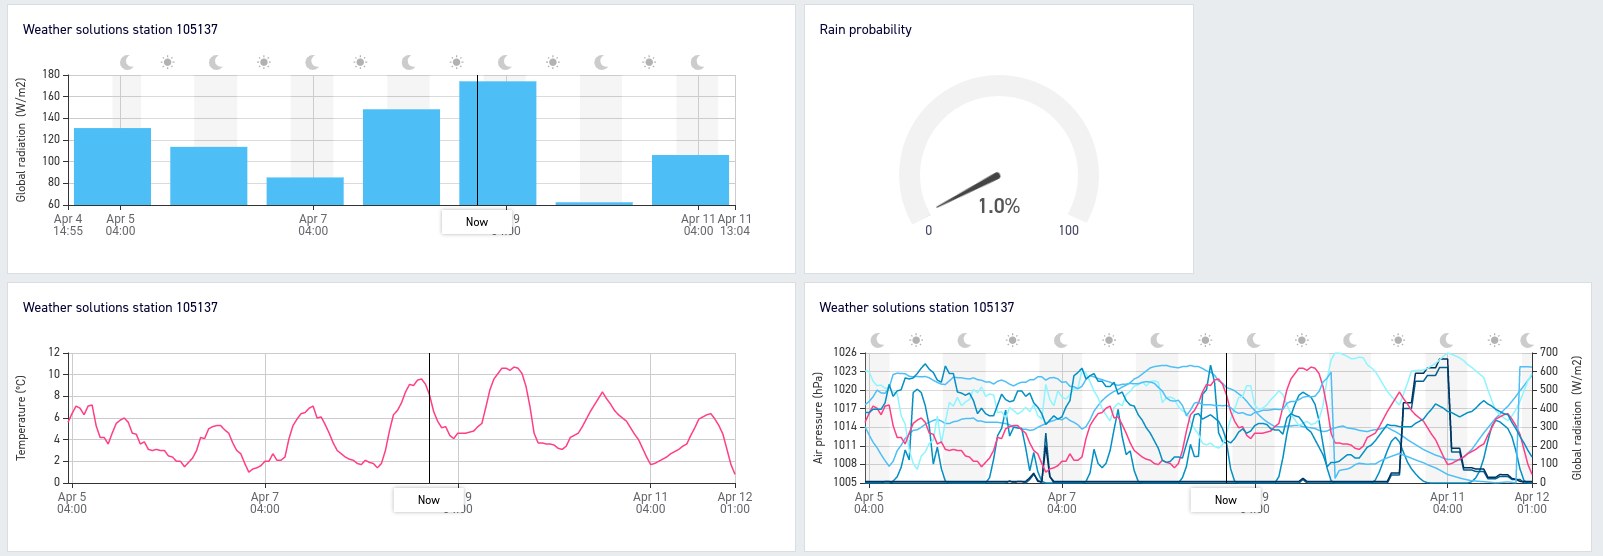
\includegraphics[width=\columnwidth]{figures/background/dashboard.png}
  \caption{Widgets in the 30MHz dashboard}
  \label{fig:bg:dashboard}
  \centering
\end{figure}

\begin{figure}[h]
  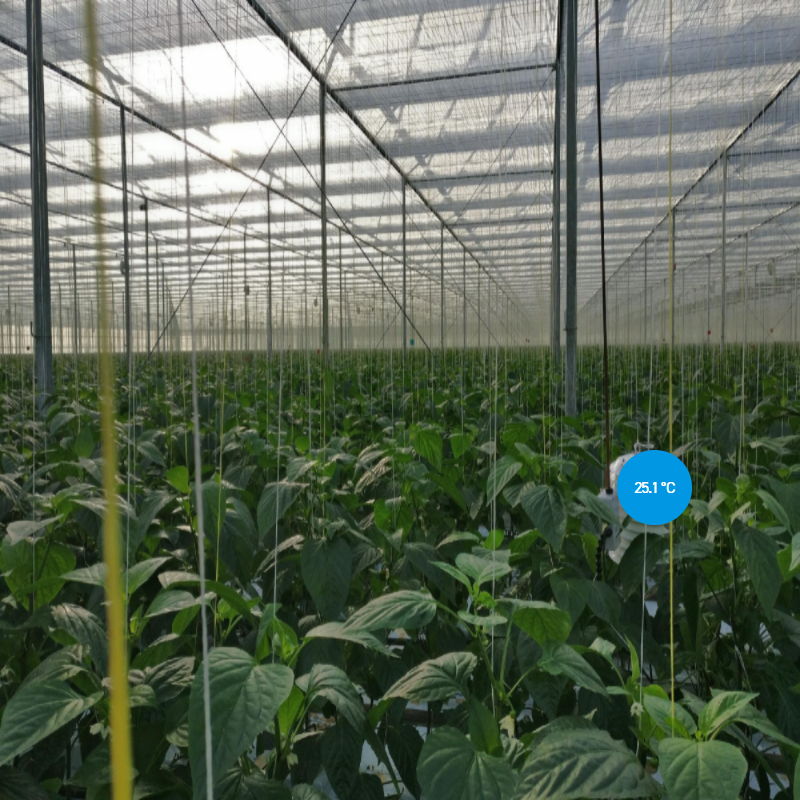
\includegraphics[width=\columnwidth]{figures/background/dashboard-img.png}
  \caption{An image widget in the 30MHz dashboard}
  \label{fig:bg:dashboard-img}
  \centering
\end{figure}

\subsection{Apps}\label{sec:bg:apps}
The data collected by 30MHz can be utilized in many ways. Companies with domain knowledge and expertise in certain areas (such as third parties) can provide customers with new insights and information that simple graphs can not. Because 30MHz itself does not have this domain knowledge and does not have the resources to create every single possible implementation of this knowledge (in the form of a widget or page in the dashboard), they decided to allow third-party developers to develop them instead. There are currently two implementations:

\begin{itemize}
  \item \emph{Widgets:} A Widget in the dashboard takes data from one or more sensors and displays it. These are made to provide information at a glance and are fairly small in screen space, as can be seen in Figure~\ref{fig:bg:dashboard}. An example would be a new way to display the amount of light a plant is getting by showing a sun icon if the plants can grow (it is daytime) and a moon icon if they are not (it is nighttime).
  \item \emph{Apps:} Full pages in the web app. These fill the entire screen (bar some 30MHz branding) and provide more rich and interactive experiences. An example would be a page where users can tune parameters (such as the number of crops, amount of watering) and see a prediction of their revenue. This prediction can be based (in part) on sensor data.
\end{itemize}

Since these apps will essentially be pages in the 30MHz dashboard and will feel like part of the platform, it is important that they follow the same design as the rest of the dashboard. A consistent design ensures that users are familiar with the apps and that visual consistency across the platform is not broken. This concept has been applied on Google's Android through Material Design~\footurl{https://material.io/} and Zendesk Garden~\footurl{https://garden.zendesk.com/} among others. Importantly, these companies all provide app developers with a set of components to help them maintain the intended design language. Such a set of components is generally referred to as a UI library.
Similarly, 30MHz wants to provide their third-party app developers with a UI library as well. In this paper, we refer to the UI library 30MHz will provide to third parties as the Cow Components UI Library (or CC UI Library). It is named after the logo of 30MHZ, a cow. There already is an internal UI library that covers the basic set of UI components (among others buttons, an input, a date picker), but since it is interwoven with other internal code, its source code can not just be provided to third-party developers. They have been written in Angular~\footurl{https://angular.io/}, meaning that any developers who wish to develop their app in a different JavaScript (JS) framework cannot do so. Looking at the most popular web frameworks in the latest Stack Overflow Developer Survey~\footurl{https://insights.stackoverflow.com/survey/2020} (2020 as of the writing of this paper), we can conclude that the chance that a developer wishes to use a different JS framework is quite large. In order to still provide developers with a CC UI library, there are two options.

\begin{itemize}
  \item Write components from scratch in a framework-agnostic format and provide them to developers. Then keep them up to date with the internal set of components by changing one as the other changes.
  \item Set up automatic conversion from the set of internal components to a framework-agnostic format.
\end{itemize}

The immediately apparent problem with the first option is that developers are maintaining two separate copies of very similar code. This causes several issues. The time spent maintaining a component is doubled. Additionally, feature differences between the Angular framework and the framework-agnostic format we choose will lead to problems. Some things that work in Angular might need workarounds in the other format and the other way around. Another issue with this option is that the components have to be written entirely from scratch. While this would be manageable for simple components such as buttons, this is unfeasible for more complex components. One such component for which this would prove difficult is the 30MHz chart component. This component is vital to the 30MHz design library, seeing as it can display the sensor data. The source code for the chart is tightly coupled with the rest of the platform, referencing about half of the source files in the dashboard through its dependencies. Rewriting all of this in another framework is wholly unfeasible and not worth the effort, leading us to explore the second option.

While the second option is not an easy one and will likely be a very complex process to set up, it will scale a lot better. Once it is set up, any new components will be automatically converted, and any changes will be propagated automatically. In the long run, this should save time. This option is the one 30MHz eventually decided on. Next, a framework-agnostic format needs to be chosen to facilitate this process.

\section{Web Components}\label{sec:bg:webcomponents}
When it comes to choosing a framework-agnostic format for a UI library, there are very few options. Looking at the literature, we find Quid~\cite{molina2019quid}, a program that allows code written in a domain-specific language (DSL) to be used to generate components in various frameworks. It currently supports the generating of Web Components~\footurl{https://developer.mozilla.org/en-US/docs/Web/Web_Components}, Stencil~\footurl{https://stenciljs.com/}, Angular and Polymer~\footurl{https://www.polymer-project.org/} components. The authors do mention it should only be used for rapid prototyping. Since it only supports a fairly small set of supported frameworks and it has the problem of requiring a DSL which the Angular code would have to be converted to, we can not use Quid as the target format.

This brings us to the other option, namely Web Components. Web Components (also known as Custom Elements) are a technology proposed in 2013~\footurl{https://www.w3.org/TR/2013/WD-custom-elements-20130514/\#about} and implemented in major browsers in 2018~\footurl{https://caniuse.com/?search=webcomponents}. It allows for the creation of custom HTML elements using JavaScript. These elements can then be used like regular HTML elements. Since every JS framework has support for native HTML elements and almost every framework has full support for Web Components~\footurl{https://custom-elements-everywhere.com/}, we can cover most JS frameworks by using Web Components as our target format.

\section{Angular Elements}\label{sec:bg:angularelements}
To perform the conversion of Angular components to Web Components, we use Angular Elements~\footurl{https://angular.io/guide/elements}. Angular Elements is a JS package that allows the conversion of Angular components to Web Components. Angular apps are typically mounted to the page by the user through a call to the \code{bootstrapModule} function. Consequently, the bootstrap component is mounted to the page. This bootstrap component is responsible for containing the rest of the application. After it is mounted, child components are mounted and rendered within its root recursively. Angular Elements works slightly differently. Components registered as Web Components through Angular Elements are instead rendered whenever an HTML element with the registered tag is added to the DOM\@. When this happens, a new root is created in place of this new HTML element. Instead of a single root in which everything is rendered (as is the case in a typical Angular app), components are all rendered in their own local root. We use Angular Elements for the conversion to Web Components in this case study since it appears to be the only package providing this task.

\begin{figure}[h]
  \caption{An example of a component that provides type hints (these hints are also referred to as intellisense)}
  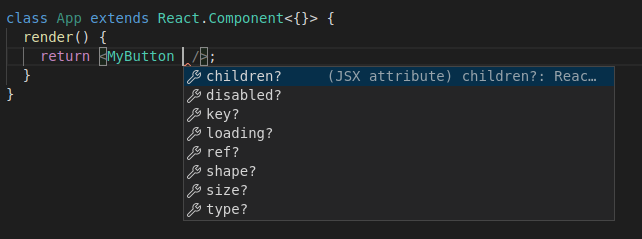
\includegraphics[width=\columnwidth]{figures/background/hinting.png}
  \label{fig:bg:hinting}
  \centering
\end{figure}

\begin{figure}[h]
  \caption{An example of a component without type hints}
  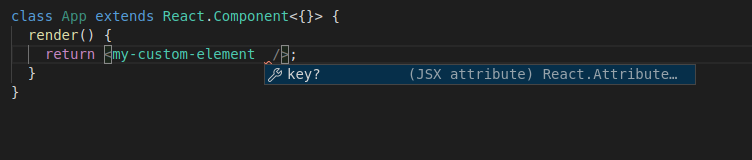
\includegraphics[width=\columnwidth]{figures/background/no-hinting.png}
  \label{fig:bg:no-hinting}
  \centering
\end{figure}

\section{Javascript frameworks}\label{sec:bg:jsframeworks}
While converting components to Web Components makes them usable in most JS frameworks, they do not provide a perfect experience. The first reason for this is them not being perfectly compatible with every JS framework. As of the writing of this paper, there are still some issues preventing them from working entirely in ReactJS~\footurl{https://reactjs.org/}, a JS framework created by Facebook in 2013. These issues mostly concern the passing of non-primitive data to the components, such as JavaScript Objects, Arrays, and Functions. The second problem is that they are not native to JS frameworks and do not integrate very well with the tooling provided by the framework. An example of type hinting provided by the framework and editor can be seen in Figure~\ref{fig:bg:hinting}. Compared to Figure~\ref{fig:bg:no-hinting}, which shows a component with no type hinting, Figure~\ref{fig:bg:hinting} provides the developer with much more information and shows them what options are available to them. Instead of searching the web for the available properties, they are provided by the element's source code and displayed by the framework tooling and editor. In order to improve the developer experience, we will provide what we will call a \emph{wrapper} for each framework. This wrapper has two functions. Firstly, it provides the tooling mentioned above. Secondly, it bridges the gap with JS frameworks that do not natively support Web Components yet. This wrapper is native to the framework, being written using the language and library the provides. This allows the framework to infer information from the wrapper's source code. Under the hood, this wrapper still uses the components in the Web Components UI library to render the components. This wrapper serves as glue code between the framework and these components. By combining the two steps of converting the original Angular components to Web Components, and the Web Components to wrappers for frameworks, we can provide developers with an experience native to their framework, even though the original source code uses Angular.

\section{UI Libraries}\label{sec:bg:ui-libraries}
As mentioned before, a set of components that adheres to one cohesive design language is generally referred to as a UI library or design library. There are two methods for implementing a design library, with one being based on doing most of the work in JavaScript and the other being based on shifting this work to CSS. The former is also referred to as a design library, with the latter being called a CSS framework. The idea of a CSS framework is to put almost all of the styles a developer will need in a single CSS file. This includes the various variations they could need. For example, a CSS library could include the \code{.padding-5} selector as well as the \code{.padding-2} selector for setting the padding of a component. Note that the number of pixels of this padding is included in the selector. This generally leads to relatively big CSS files, which may or may not be tree shaken. This is in contrast to JavaScript-based UI libraries, which generally use per-component stylesheets instead of global stylesheets. They also tend to shift numbers and sizes to JavaScript or HTML\@. For example the same padding as above could be applied through a property, i.e. \code{<my-component padding="2"/>} or \code{<my-component padding="5"/>}. This approach has the advantage of a more per-component focus, more flexibility, and options that are easier to discover. However, compared to CSS frameworks, JS-based UI libraries are significantly slower. The CSS frameworks generally only append an element to the DOM and apply some pre-computed set of classes to them, meaning they only interact with the swift JavaScript APIs that are native to the browser. JS-based UI libraries, on the other hand, generally have to run a lot more code. Since this performance difference is important when it comes to measurements, a given library being a UI library or CSS framework, is mentioned later.

\section{Related Work}\label{sec:related-work}

There are various fields in which the related work is important to us in this paper. Namely related work in the area of UI Libraries, Angular Elements (and the accompanying process of converting to Web Components), related work on Web Components themselves, and related work on the creation of wrappers around Web Components to target JS frameworks.

\subsection{UI Libraries}
We found a few studies that cover the area of UI libraries. In~\cite{ky2019ui}~\cite{annala2017documentation}~\cite{mrazcomponent}, the authors all build UI libraries. They focus mostly on the technologies used, how they work, and how they contribute to the building of the UI library. Looking at blog posts, we find numerous posts on Web Components. In these blog posts~\footurl{https://www.toptal.com/designers/ui/design-framework}~\footurl{https://dev.to/giteden/building-a-ui-component-library-for-your-startup-4cek}~\footurl{https://www.emergeinteractive.com/insights/detail/how-to-ux-ui-design-system-component-library/}~\footurl{https://codeburst.io/building-an-awesome-ui-component-library-in-2020-a85cb8bec20}~\footurl{https://itnext.io/building-a-scalable-ui-component-library-4607de91955a}, the authors provide guidance in setting up and creating a UI library. These blog posts mainly concern the basics, explaining how to get started with the process. We also find numerous examples of UI libraries. Some examples are Svelte Material UI~\footurl{https://sveltematerialui.com/} (written in Svelte), React Bootstrap~\footurl{https://react-bootstrap.github.io/} (React), Angular Material~\footurl{https://material.angular.io/} (Angular), Wired Elements~\footurl{https://wiredjs.com/} (Web Components), Onsen~\footurl{https://onsen.io/} (multi-framework), and SyncFusion~\footurl{https://www.syncfusion.com/}. For all but the SyncFusion, the source code is freely available on GitHub, allowing us to draw inspiration from it and look at how various problems were solved in different UI libraries.

\subsection{Angular Elements}
Research on the area of Angular Elements is very sparse. In our search, we only found a single paper on this subject. In~\cite{armengol2020development}, Angular Elements is used to convert form components to Web Components so that they can be rendered dynamically. On the other hand, blog posts on this area are numerous. In various blog posts~\footurl{https://netbasal.com/understanding-the-magic-behind-angular-elements-8e6804f32e9f}~\footurl{https://medium.com/kitson.mac/wrapping-an-angular-app-in-a-custom-element-web-component-angular-element-in-4-simple-steps-ded3554e9006}~\footurl{https://medium.com/@smarth55/angular-elements-use-them-everywhere-including-your-angular-app-697f8e51e08d}~\footurl{https://blog.piotrnalepa.pl/2020/02/02/how-to-convert-angular-component-into-reusable-web-component/}~\footurl{https://medium.com/swlh/angular-elements-create-a-component-library-for-angular-and-the-web-8f7986a82999}~\footurl{https://www.thirdrocktechkno.com/blog/angular-elements/}~\footurl{https://juristr.com/blog/2019/04/intro-to-angular-elements/}~\footurl{https://studiolacosanostra.github.io/2019/07/19/Build-a-reusable-Angular-library-and-web-component/}~\footurl{https://blog.bitsrc.io/using-angular-elements-why-and-how-part-1-35f7fd4f0457}~\footurl{https://www.techiediaries.com/angular/angular-9-elements-web-components/}~\footurl{https://indepth.dev/posts/1116/angular-web-components-a-complete-guide}~\footurl{https://indepth.dev/posts/1228/web-components-with-angular-elements}, the authors explain how to set up Angular Elements and how to use it to create a new component library. These blog posts mostly focus on creating new components or converting simple components through Angular Elements, not so much on converting larger and more complex components. They all use new and empty projects, contrary to two other blog posts~\footurl{https://blog.nrwl.io/upgrading-angularjs-to-angular-using-elements-f2960a98bc0e}~\footurl{https://medium.com/capital-one-tech/capital-one-is-using-angular-elements-to-upgrade-from-angularjs-to-angular-42f38ef7f5fd}. The authors use Angular Elements to convert existing AngularJS (an older version of Angular) components to the newer Angular. They do this by converting the source code of existing AngularJS components to Angular source code. By itself, this would break since the application root still runs on AngularJS and is unable to handle Angular code. By using Angular Elements to convert the Angular code into Web Components, the Web Components are able to run inside the AngularJS root. This is thanks to the low-level nature of Web Components, allowing any framework that can render HTML elements to use them. Through this iterative process, they are able to convert components one by one, converting the root component once all of its children have been converted as well.

Unfortunately, we were unable to find any related work on the conversion of complex Angular components to Web Components through Angular Elements. Related work seems to focus mostly on small get-started style projects. In the cases where they do focus on more complex projects, it seems like the only use is the conversion from AngularJS to Angular.

\subsection{Web Components}
\todo{Web Components section}

\subsection{JS Framework Wrappers}
We were unable to find any research on JS framework wrappers. This does not seem to be a problem that has been tackled very often, at least in literature. On the website \emph{custom-elements-everywhere.com}~\footurl{https://custom-elements-everywhere.com/}, the authors keep track of the current usability of Web Components in various JS frameworks. Notably, the ReactJS framework does not fully support Web Components at the time of writing for this paper. In ReactJS, non-primitive values (such as Objects, Arrays, and Functions) can not be passed to Web Components, along with some other issues. As such, it is the only framework that needs a wrapper for the UI library to function at all. Looking at how to fix this issue, we find some proposed solutions in a blog post~\footurl{https://itnext.io/handling-data-with-web-components-9e7e4a452e6e}. In this blog post, the author explores various options to tackle this problem of passing non-primitive data.
\chapter{Study Design}\label{chap:design}

\section{Research questions}
Our goal in this paper is to evaluate the effectiveness of migrating Angular components to Web Components. Based on this goal, a single research question has been devised:
\\
\\
\textbf{RQ1: How technically viable is the process of migrating Angular components to Web Components?}
\\
In answering this research question, we assess whether the migration process is possible at all, what a possible performance impact could be, and how the result relates to other component libraries in the field
\\

\section{Metric definitions}
In order to answer the above research questions, we need to define metrics. These allow us to compare the resulting Web Component library both to the UI library and to other UI libraries. This allows us to get a better understanding of the quality and performance of the created Web Component library relative to other UI libraries. We can divide the metrics used into two categories. The first is measuring the effectiveness of the resulting CC UI library. In order to do this, we compare the components in the CC UI library to the Angular components they originate from, as well as to various UI libraries. We perform this comparison using various metrics at both component granularity and at UI library granularity. A full list of these metrics, as well as a brief description, can be seen in Table~\ref{tab:design:metrics}. A detailed explanation of these metrics follows.


\begin{table}[h]
  \tiny
  \begin{tabularx}{\textwidth}{|l|l|l|X|}
    \toprule
    \textbf{ID} & \textbf{Metric}        & \textbf{Granularity}             & \textbf{Description}                                                                                                              \\ \midrule
    SC          & Structural complexity  & Component                        & The number of import statements for a component. Collected for a source file and all of its dependencies for up to two iterations \\ \hline
    CC          & Cyclomatic complexity  & Component                        & A quantitative measure of the number of linearly independent paths through a program's~\cite{1702388}                             \\ \hline
    LOC         & Lines of code          & Component                        & The number of lines of code in a given component's source file                                                                    \\ \hline
    MA          & Maintainability        & Component                        & A derivative based on complexity, lines of code and Halstead volume~\cite{halstead1977elements}                                   \\ \hline
    RT          & Render Time            & Component                        & The render time of a given component                                                                                              \\ \hline
    SI          & Size                   & UI Library                       & The file size of the bundled up library                                                                                           \\ \hline
    LT          & Load Time              & UI Library                       & Parsing and running time of the bundled up library in the browser (without download time)                                         \\ \hline
    NOC         & Number of Components   & UI Library                       & The number of components in a UI library                                                                                          \\ \hline
    FC          & First Paint            & UI Library (cow-components only) & First paint event of the browser                                                                                                  \\ \hline
    FCP         & First Contentful Paint & UI Library (cow-components only) & First paint event of the browser that includes content for the user  (text, images, etc.)                                         \\
  \end{tabularx}
  \caption{Metrics used in this study}
  \label{tab:design:metrics}
\end{table}

\subsection{Source code metrics}
The first set of metrics, namely structural complexity, cyclomatic complexity, lines of code, and maintainability, are metrics that are recommended by Martinez-Ortiz \etal{}~\cite{martinez-ortiz2016quality} as described in Section~\ref{sec:related-work:metrics}. We use these metrics to compare the quality of our Web Components to other Web Components. We follow almost all recommendations by the paper, including collecting the structural complexity up to a depth of two. Note that we do things slightly differently from the paper. We also keep track of the lines of code metric, which the authors do not. We do not use this to compare the quality of Web Components but instead we use it to get a rough overview of the complexity of various UI libraries. Note that we are also not using all metrics recommended by the authors. The metrics we are not using are the completeness (i.e.~how complete the information displayed to the user is) and consistency(i.e.~how long it takes for data to update across different replicas) metrics. We are not using completeness because it does not apply at the level at which the CC UI library operates. All of our components are 100\% complete, as well as the components of the UI libraries we compare the CC UI library to. As such, it does not make for a very interesting metric. This metric is very effective when more complex components such as entire pages are concerned, but that is not the case here. We also do not use the consistency metric. The reason for this is relatively simple, namely that we do not have any components with the ability to update across different replicas. The same goes for the UI libraries with which we compare it.

\subsection{Size}
The size metric aims to measure the theoretical impact of loading the UI library over the network. We measure this at UI library level granularity since the contributions of individual components are very hard to measure. This should serve as a good indication of the relative network loading time of UI libraries without introducing the variable of network speed. In order to differentiate between a relatively large library and a library that has many components, we also keep track of the number of components metric.

\subsection{Load Time}
The load time metric aims to provide a measure of the real impact of a UI library on the page by measuring the real-world load time. The load time we measure is the load time of the main JS bundle. This contains the code needed to register the components to the page, as well as the rendering. Note that we only measure the parsing time and running time of the JavaScript bundle. We explicitly exclude the download time from this metric since this is already captured in SI\@. A more in-depth definition of how this metric is captured is discussed in section~\ref{sec:experimental-setup:load-time}.

\subsection{First Paint \& First Contentful Paint}
The first paint metric, along with the FCP metric, are on just the cow-component UI libraries. These metrics give us an indication of the real-world load time of a page containing the CC UI library and the original components. We use these metrics to evaluate how the paint time of the UI libraries has changed after its conversion to Web Components and its later conversion to JS framework wrappers. While these metrics do not serve as a perfect way to measure the perceived load time of a page, as discussed in Section~\ref{sec:related-work:load-time}, they should serve as an excellent comparison between the various UI libraries. Since each of them contains the exact same content and is derived from the exact same source code, imperfections in these metrics are applied to all test subjects equally.

\subsection{Render Time}
Finally, the render time metric aims to capture the duration of the render cycle. We will define this render time as the time between setting the component's visibility to true and the browser being done with the rendering process. If the render time of components in the CC UI library is significantly higher than components in other UI libraries or the Angular components they originate from, the performance impact of migrating Angular components to Web Components will be too significant. If it is slightly higher, the same, or lower, we can conclude that the performance impact is minimal.

In order to obtain an objective measurement of the rendering time that is independent of user perception, we chose to measure the render time of individual components. Since the components we use in our comparisons all load in a single stage (they are either not visible or visible), there is no loading state that could cause ambiguity.

\section{Metric targets}
In order to get a sense of the state of the CC UI library, we need to compare it to other UI libraries. To do so, we have gathered a list of various UI libraries targeting the most popular JS frameworks. These most popular frameworks are React, Angular, Vue, and Svelte~\footurl{https://2020.stateofjs.com/en-US/technologies/front-end-frameworks/}. This way, we can compare the wrapper targeting a specific JS framework with UI libraries that also target that JS framework, allowing us to observe the influence of the framework itself on the various metrics. These UI libraries were gathered by searching for the terms ``Design Library'', ``UI Library'', ``javascript UI Library'', ``Svelte UI library'', ``React UI Library'', ``Vue UI Library'', ``Angular UI Library'', and ``Web Component UI Library'' on Google. We then added any UI library to the list that we came across, either by finding it as a direct result or it being mentioned in a blog post or article. A list of the UI libraries we found and the number of stars on their GitHub page can be found in Table~\ref{tab:design:ui-libraries}. While this is not a complete list of all UI libraries, we feel like it is an accurate representation of the most popular UI libraries since it contains all of the biggest UI libraries, as confirmed by the numerous blog posts listing them in order. In order to get a reasonably accurate representation of libraries using each JS framework, we selected the three UI libraries with the most GitHub stars per JS framework. The list of included UI libraries can also be seen in Table~\ref{tab:design:ui-libraries}. In addition to comparing the CC UI library against other UI libraries, we also compare it against the Angular components from which they originate. We do this by applying our metrics to the 30MHz dashboard and the relevant components within it.

Since the components included in the selected UI libraries vary greatly, we can not make a proper comparison between individual components of the UI library. For example, a button component can not be compared with a date picker component since date pickers tend to be more complex. Higher rendering times can not be attributed to the UI library running it but to the component itself. In order to be able to compare every UI library, we have selected a set of basic components that are available in every UI library. These are the Button, Input, and Switch (or Checkbox). Since every UI library contains all of these, we can compare the metrics for a single component across all UI libraries. We only apply the various metrics to these three components in each UI library. We also include a stripped-down version of the CC UI library in the set of UI libraries of which we gather metrics. This version only contains the three components mentioned above and allows for a fair comparison with other UI libraries. The reason for this is further explained in Section~\ref{sec:experimental-setup:size}.

\begin{table*}[t]
  \tiny{}
  \begin{tabularx}{\textwidth}{p{0.15\textwidth} |p{0.1\textwidth} | p{0.18\textwidth} | p{0.07\textwidth} | p{0.1\textwidth} |p{0.4\textwidth}  }
    \toprule
    \textbf{UI Library}     & \textbf{Github Stars}   & \textbf{JS Framework} & \textbf{Included} & \textbf{Version} & \textbf{Website}                                                                 \\ \midrule
    Svelte Material UI      & 1.6k                    & Svelte                & Yes               & 2.0.0            & \url{https://sveltematerialui.com/}                                              \\ \hline
    Smelte                  & 889                     & Svelte                & Yes               & 1.1.2            & \url{https://smeltejs.com/}                                                      \\ \hline
    Svelte-MUI              & 237                     & Svelte                & Yes               & 0.0.3-7          & \url{https://svelte-mui.ibbf.ru/}                                                \\ \hline
    Svelteit                & 51                      & Svelte                & No                & -                & \url{https://docs.svelteit.dev/}                                                 \\ \hline
    Material UI             & 67.1k                   & React                 & Yes               & 5.0.0-alpha.28   & \url{https://material-ui.com/}                                                   \\ \hline
    React Bootstrap         & 19.2k                   & React                 & Yes               & 1.5.2            & \url{https://react-bootstrap.github.io/}                                         \\ \hline
    React Semantic UI       & 12.2k                   & React                 & Yes               & 2.0.3            & \url{https://react.semantic-ui.com/}                                             \\ \hline
    Evergreen               & 10.6k                   & React                 & No                & -                & \url{https://evergreen.segment.com/}                                             \\ \hline
    Rebass                  & 7.2k                    & React                 & No                & -                & \url{https://rebassjs.org/}                                                      \\ \hline
    Grommet                 & 7.1k                    & React                 & No                & -                & \url{https://v2.grommet.io/}                                                     \\ \hline
    Baseweb                 & 6.2k                    & React                 & No                & -                & \url{https://baseweb.design/}                                                    \\ \hline
    Ant Design              & 5.3k                    & React                 & No                & -                & \url{https://ant.design/}                                                        \\ \hline
    Elemental UI            & 4.3k                    & React                 & No                & -                & \url{http://elemental-ui.com/home }                                              \\ \hline
    Zendesk Garden          & 858                     & React                 & No                & -                & \url{https://garden.zendesk.com/}                                                \\ \hline
    Shards React            & 649                     & React                 & No                & -                & \url{https://designrevision.com/docs/shards-react/getting-started }              \\ \hline
    Angular Material        & 21.3k                   & Angular               & Yes               & 12.0.0-next.5    & \url{https://material.angular.io/}                                               \\ \hline
    NG-Bootstrap            & 7.7k                    & Angular               & Yes               & 9.1.0            & \url{https://ng-bootstrap.github.io/\#/home }                                    \\ \hline
    NGX-Bootstrap           & 5.3k                    & Angular               & Yes               & 7.0.0-rc.0       & \url{https://valor-softw2are.com/ngx-bootstrap/\#/ }                             \\ \hline
    NG-Lightning            & 886                     & Angular               & No                & -                & \url{https://ng-lightning.github.io/ng-lightning/\#/ }                           \\ \hline
    Alyle                   & 236                     & Angular               & No                & -                & \url{https://alyle.io/}                                                          \\ \hline
    Blox Material           & 143                     & Angular               & No                & -                & \url{https://material.src.zone/}                                                 \\ \hline
    Mosaic                  & 117                     & Angular               & No                & -                & \url{https://mosaic.ptsecurity.com/button/overview }                             \\ \hline
    Element                 & 49.8k                   & Vue                   & Yes               & 1.0.2-beta.40    & \url{https://element-plus.org/\#/en-US}                                          \\ \hline
    Vuetify                 & 30.2k                   & Vue                   & Yes               & 2.4.9            & \url{https://vuetifyjs.com/en/}                                                  \\ \hline
    Quasar                  & 18.3k                   & Vue                   & Yes               & 1.15.10          & \url{https://quasar.dev/ }                                                       \\ \hline
    Ant Design Vue          & 14.1k                   & Vue                   & No                & -                & \url{https://2x.antdv.com/docs/vue/introduce }                                   \\ \hline
    Bootstrap Vue           & 13.1k                   & Vue                   & No                & -                & \url{https://bootstrap-vue.org/ }                                                \\ \hline
    Vue-material            & 9.3k                    & Vue                   & No                & -                & \url{https://vuematerial.io/ }                                                   \\ \hline
    Buefy                   & 8.6k                    & Vue                   & No                & -                & \url{https://buefy.org/ }                                                        \\ \hline
    Vuesax                  & 5k                      & Vue                   & No                & -                & \url{https://vuesax.com/ }                                                       \\ \hline
    Chakra                  & 1.1                     & Vue                   & No                & -                & \url{https://vue.chakra-ui.com/ }                                                \\ \hline
    Fish UI                 & 867                     & Vue                   & No                & -                & \url{https://myliang.github.io/fish-ui/ }                                        \\ \hline
    Wired Elements          & 8.5k                    & Web Components        & Yes               & 1.0.0            & \url{https://wiredjs.com/}                                                       \\ \hline
    Clarity Design          & 6.2k                    & Web Components        & Yes               & 5.1.0            & \url{https://clarity.design/}                                                    \\ \hline
    Fast                    & 5.6k                    & Web Components        & Yes               & 1.8.0            & \url{https://www.fast.design/}                                                   \\ \hline
    Material Web Components & 2.5k                    & Web Components        & No                & -                & \url{https://github.com/material-components/material-components-web-components } \\ \hline
    UI5                     & 887                     & Web Components        & No                & -                & \url{https://sap.github.io/ui5-webcomponents/}                                   \\ \hline
    Vaadin                  & 17                      & Web Components        & No                & -                & \url{https://vaadin.com/}                                                        \\ \hline
    Onsen                   & 8.3k                    & Multi-Framework       & Yes               & 2.11.2           & \url{https://onsen.io/}                                                          \\ \hline
    Primefaces (Angular)    & 1.3k                    & Multi-Framework       & Yes               & 11.3.2-SNAPSHOT  & \url{https://www.primefaces.org/primeng/}                                        \\ \hline
    Primefaces (React)      & 1.3k                    & Multi-Framework       & Yes               & 6.2.2-SNAPSHOT   & \url{https://www.primefaces.org/primereact/}                                     \\ \hline
    Primefaces (Vue)        & 1.1k                    & Multi-Framework       & Yes               & 3.3.6-SNAPSHOT   & \url{https://www.primefaces.org/primevue/}                                       \\ \hline
    Syncfusion              & unknown (not on github) & Multi-Framework       & No (paid)         & 1.0.0            & \url{https://www.syncfusion.com/}
  \end{tabularx}
  \caption{Collected UI libraries, the number of github stars and whether they were included in the study}
  \label{tab:design:ui-libraries}
\end{table*}

\section{Analysis of results}
In order to compare the collected measurements, we use the median value over a set of measurements. Compared to the average, the median minimizes the impact of outliers in a data set. Since the measurements we collect are likely to have outliers in them due to the nature of time-sensitive measurements, this statistical value is likely to be a better choice.
\chapter{Experimental Setup}\label{chap:experimental-setup}
We now describe how each of the metrics is being captured and what parameters are used.

\section{Gathering components}\label{sec:experimental-setup:gathering-components}
The SC, CC, LOC, and MA metrics are captured from the source files of components. In order to gather these source files, we do the following: We set up an automatic script that gathers the source files of components on a per-library basis. Since most UI libraries follow the convention of storing each component in a single folder or file in a source folder (generally called \ver{src/} or \ver{components/}), this process is fairly simple. In order to provide a fair comparison, we always select the largest source file for components as the entry point. Some UI libraries use a simple index file that re-exports the actual source file as the entry point. If this file were to be used as the entry point, it would result in an unrealistic depiction of the component source. Since the UI libraries in this study always contain a single big source file, this did not result in any situations where the entry point was ambiguous.

\section{Structural Complexity}
The structural complexity is gathered by capturing the number of imports in a given source file recursively up to a depth of two, as recommended in~\cite{martinez-ortiz2016quality}. To gather these imports, we use the \ver{typescript}\footurl{https://www.npmjs.com/package/typescript} JS package. This package is able to generate an AST or abstract syntax tree of the file. An AST is an in-memory representation of source code. It categorizes the semantic meaning of each expression as a tree, denoting relations between nodes in the tree. By iterating over this tree, we can find the imports. We then follow these imports and apply the same process, filtering out any duplicates.

Similar to~\cite{martinez-ortiz2016quality}, we only apply this process to the JS source code of a component, not the HTML source code. In the case of Svelte and Vue components, we separate the file into its JS code and HTML code and apply the process to the JS code only. Code using ReactJS is written using either plain JavaScript or JSX. JSX is a superset of JavaScript that supports the describing of HTML elements in JavaScript. Since the \ver{typescript} package has built-in support for JSX, we do not need to separate or modify this code.

\section{Cyclomatic Complexity, Maintainability, Lines of Code}
In order to capture the cyclomatic complexity, maintainability metrics, and lines of code metrics, we input the file into the \ver{ts-complex}\footurl{https://www.npmjs.com/package/ts-complex} JS package. This package is able to calculate the cyclomatic complexity, maintainability, and lines of code metrics for a given source file. Note that the lines of code metric does not capture the raw number of lines but instead filters out any comments, aiming to capture just the lines with actual code.

\section{Machine specifications}\label{sec:experimental-setup:machine-specs}
All experiments are performed on a machine with an AMD Ryzen 5 4600H six-core processor and 16GB of RAM. This machine is running Linux 5.11.15 using the Arch Linux distribution~\footurl{https://archlinux.org/} with the \code{mitigations=auto} kernel parameter. All experiment data is loaded from an M.2 SSD. Since these experiments are partially timing-specific, the timing-specific experiments are run sequentially and with minimal background tasks. We achieved a state of minimal background tasks by closing off all non-essential tasks found in the process manager. This should eliminate the effect of experiments on each other and ensure the CPU can always dedicate a single core to the running experiment. Since this machine has six cores, it should easily be able to dedicate one of them to the experiments at all times. Finally, since all experiments were run in one go, the test environments for all tests are identical.

\section{Time-sensitive metrics}\label{sec:experimental-setup:time-sensitive-metrics}
For all time-sensitive metrics (metrics that measure time), we take a few steps to improve their accuracy. We first of all artificially slow down the speed of the processor by a factor of \slowdownFactor{} by using the \code{Emulation.setCPUThrottlingRate} command~\footurl{https://chromedevtools.github.io/devtools-protocol/tot/Emulation/\#method-setCPUThrottlingRate} in the browser. We then divide the measured number by this scale, normalizing the value. Additionally, we perform every time-sensitive measure \numMeasures{} times. This allows us to get a good overview of the spread of the measured values, as well as reducing the effect of variations in hardware performance and software influences. Finally, we randomize the order in which tests are run. We do this by creating a queue of all to-be-ran time metrics. Every item in the queue is a single-time metric test for a single bundle, meaning every metric bundle combination is in the queue \numMeasures{} times. This queue is then shuffled, after which the individual items are executed. While we already made sure to reduce the number of running processes on the benchmark computer, this should ensure that any temporary differences in available processing time should be smoothed out.


\section{Size}\label{sec:experimental-setup:size}
In capturing the size metric, we need to pay attention to several influential factors. The first factor is that the source code of files is split up into multiple files, some of which are not actually used at runtime. Examples of this include files used during testing and type definition files. Additionally, it is possible that unreachable code does not make it into the bundle because it will not be executed. The process by which code that is not going to be executed is excluded from the resulting bundle is called \emph{tree shaking} and is discussed later. The fact that the source code contains unreachable code means that the size of the source code is not representative of the code that is actually being used. Additionally, the UI library will have dependencies outside of its source code that also need to be included. To get around these issues, we use a JavaScript bundler. A bundler is a program that bundles all of the source code of a given project into a single file, including dependencies and source files that are being used, and excluding unreachable files or code. We use the \ver{esbuild}\footurl{https://esbuild.github.io/} bundler for this process.

Another influential factor in determining the size is the way in which the source code is written. A file containing many comments is larger than a file containing no comments. An increased number of comments in a file does not necessarily indicate increased complexity; if anything, it indicates the opposite. Similarly, longer variable names increase the size as well. To eliminate this factor, we apply \emph{minification} to our bundle. Minification strips out any non-code text from a bundle and reduces the size of the code to the minimum that is needed.

The final influential factor is the number of components and the type of components. A UI library with five components will generally be smaller than a UI library with thirty components. Even when we account for this difference by capturing the number of components, the result will still be influenced by the types of components the UI library contains. For example, if two UI libraries are the same except that one of them contains a complex chart component, the chart heavily skews the average size of a component. This is the case even though any given component in the other library is the same size; the chart library just has different types of components. To get around this issue, we make sure to construct a bundle containing the same three types of components for every UI library. We then make use of \emph{tree shaking} to exclude other components from the bundle. Tree shaking is the process by which unused code is removed from a JS bundle, effectively reducing its contents to just code that is reachable. By including the same three types of components into the bundle for every UI library, we can create bundles containing the same functionality and nothing more. This eliminates the influence of bigger or smaller components that are also available in the UI library since they are excluded from the bundle entirely.

The tree-shaking process is applicable to the UI libraries against which we are comparing the CC UI library. However, it is not applicable to the CC UI library itself. This is the case because every component is registered as a Web Component simply by loading the library, which means that every component is used. Tree shaking is then unable to remove any components from the bundle, leading to a relatively larger bundle. This would lead to the CC UI library having a much larger size than other UI libraries. To provide a fair comparison, we add a stripped-down version of the CC UI library to the set of UI libraries against which we are comparing. This stripped-down version only contains the three basic components, and as such, allows for fairer size comparison against other UI libraries.

After these factors are taken care of, the process of capturing the size metric is as easy as getting the file size of the resulting bundle.

\section{Load Time}\label{sec:experimental-setup:load-time}
For the load time metric, we capture the parse- and runtime of the JS bundle described in Section~\ref{sec:experimental-setup:size}. We explicitly exclude the network load time of the bundle. In order to collect this metric, we use the \ver{puppeteer}\footurl{https://github.com/puppeteer/puppeteer} JS package. This package allows the running of and programmatic control over a headless instance of the Google Chrome browser~\footurl{https://www.google.com/intl/en_us/chrome/} (a headless browser is a browser without a graphical user interface). We set up an empty webpage containing just the JS bundle whose load time we wish to measure. We then enable the Chrome profiler~\footurl{https://developer.chrome.com/docs/devtools/evaluate-performance/} for the page. The Chrome profiler is a profiler built into the Google Chrome browser that allows for the measuring of various metrics during page execution. For example, it is able to measure the run time of JavaScript code and various browser-specific tasks such as painting, compositing, and rendering. We now load the page, stop the profiler and collect the results. We then look for the \code{EvaluateScript} event in the resulting trace events. This contains the time taken evaluating the given bundle. An example of such a trace can be seen in Figure~\ref{fig:experimental-setup:load-time}.

\begin{figure}[htbp]
  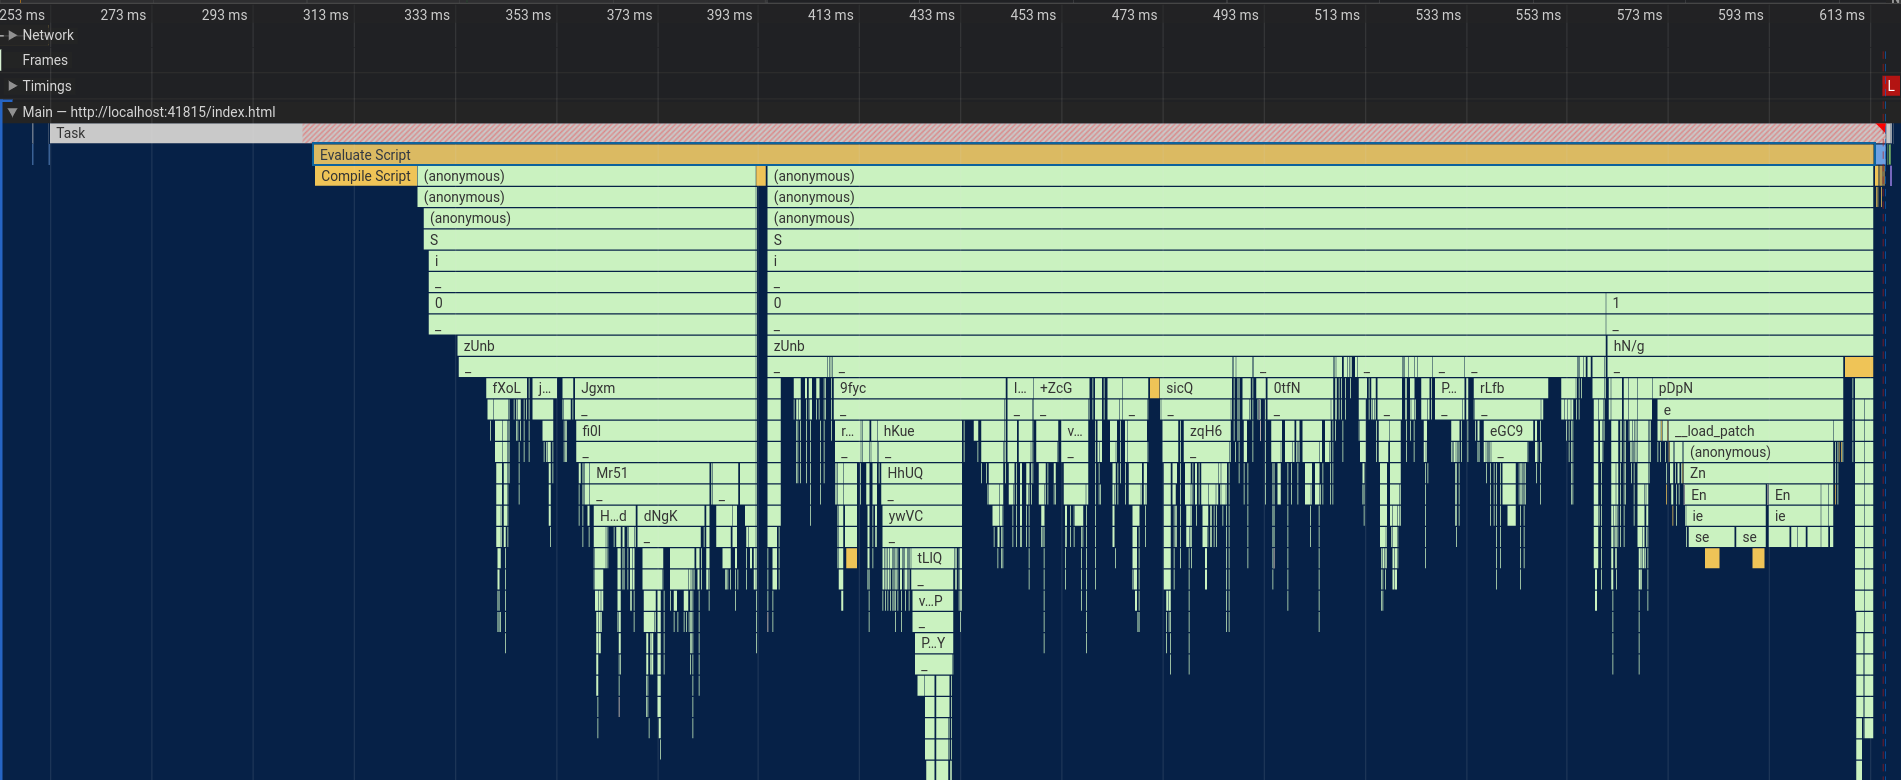
\includegraphics[width=\columnwidth]{figures/experimental-setup/load-time.png}
  \caption{An example of a Chrome profiler trace performed during a bundle load. The orange bar labeled ``Evaluate Script'' indicates the total load time and spans 308.54ms.}
  \label{fig:experimental-setup:load-time}
  \centering
\end{figure}

\section{Render Time}
We capture the render time metric by using the puppeteer package as well. We prepare a JS bundle containing the three basic components and an exposed function that allows them to be rendered on-demand. This function is JS framework-specific since every JS framework has a different method of conditional rendering. The rendering methods for the various frameworks can be seen in Listings~\ref{lst:appendix:react-set-visible},\ref{lst:appendix:angular-set-visible-html},~\ref{lst:appendix:angular-set-visible-js},~\ref{lst:appendix:svelte-set-visible},~\ref{lst:appendix:web-components-set-visible}. We then load the page in a puppeteer browser, enable the profiler, and call the function that renders a given component. We wait for a few seconds, after which we assume the component to be fully rendered. If our assumption turns out to be wrong and the component is not done rendering at time of looking for the end event, we will be unable to find the end event, and metric collecting will fail. We then increase this timeout and try it again. We then iterate through the captured performance trace and look for the time difference between two events. The first event is the calling of the function mentioned above. The second event is the last composite event that has a paint event before it. We repeat this process three times per component (on top of the \numMeasures{} mentioned in Section~\ref{sec:experimental-setup:time-sensitive-metrics} for a total of ninety measurements), \numMeasures{} measurements with a single instance of the component, \numMeasures{} measurements with 10 instances, and \numMeasures{} measurements with 100 instances. This allows us to measure a more realistic scenario where multiple components are rendered at once, as well as eliminating any performance impacts on just the very first component.

We chose the last composite event that has a paint event before it for the following reason. The chrome browser updates the view through a pipeline process. The complete pipeline can be seen in Figure~\ref{fig:experimental-setup:pipeline}. This process always starts with a JS, CSS, or HTML change. Then it performs a different set of pipeline events depending on what changed.

\begin{figure}[htbp]
  
\includegraphics[width=\columnwidth]{figures/experimental-setup/render-pipeline.jpg}
  \caption{The render pipeline in chrome.}
  \source{\url{https://developers.google.com/web/fundamentals/performance/rendering}}
  \label{fig:experimental-setup:pipeline}
  \centering
\end{figure}

\begin{itemize}
  \item \emph{Layout:} If a layout property such as the element's dimensions changes, the entire pipeline is run.
  \item \emph{Paint:} If a paint-only property such as a color changes, all but the layout stages run.
  \item \emph{Animation:} If a property that neither layout nor paint changes, only the JavaScript, style, and composite stages run. This pipeline is generally run when an animation is active.
\end{itemize}

In capturing the render time, we want to capture the time until a component reaches its final state. We need to define this final state for all components. While this state is fairly simple to define and is static for most components, it can also be a dynamic final state. For example, a loading spinner or a component that contains a canvas will at some reach its final state but will still be visually changing. The time between the component not being visible and it reaching its final state are spent in the Layout and Paint stages, while the time after it is spent in the Animation stage. Since we want to capture only the time until the final state, we only care about the Layout and Paint stages. The only difference between these two stages and the Animation stage is that the Animation stage ends with a composite event without a paint event before it, and the other two do not. We use this to our advantage by looking for the last composite event that has a paint event before it. We can not just take the last paint event since the composite event is still part of the pipeline and is technically part of the render stage. When we take the time between the calling of the function that starts the rendering and this event, we are able to capture the time a component takes to render perfectly. A visual representation of this rendering process can be seen in Figure~\ref{fig:experimental-setup:render-time-start} and Figure~\ref{fig:experimental-setup:render-time-end}.

\begin{figure}[htbp]
  \centering{}
  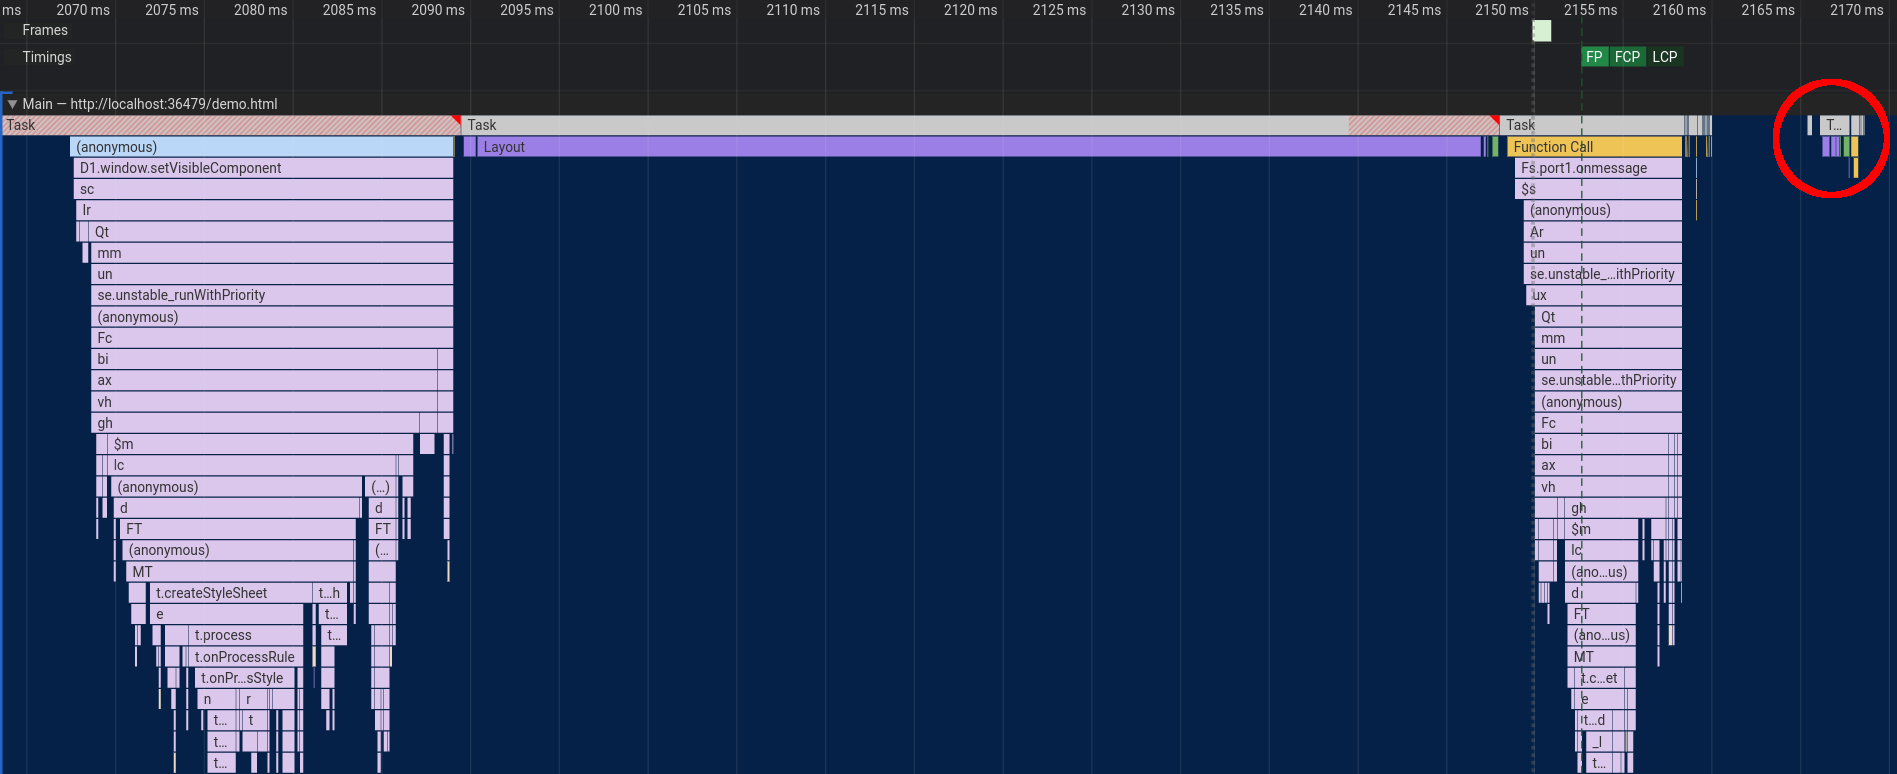
\includegraphics[width=0.8\columnwidth]{figures/experimental-setup/render-time-highlighted.png}
  \caption{An example of a Chrome profiler trace performed during the render of a component. The bar labeled ``window.setVisibleComponent'' indicates our start time. The end time falls within the red circle, a zoomed in version of which can be seen in Figure~\ref{fig:experimental-setup:render-time-end}.}
  \label{fig:experimental-setup:render-time-start}
  \centering
\end{figure}

\begin{figure}[htbp]
  \centering{}
  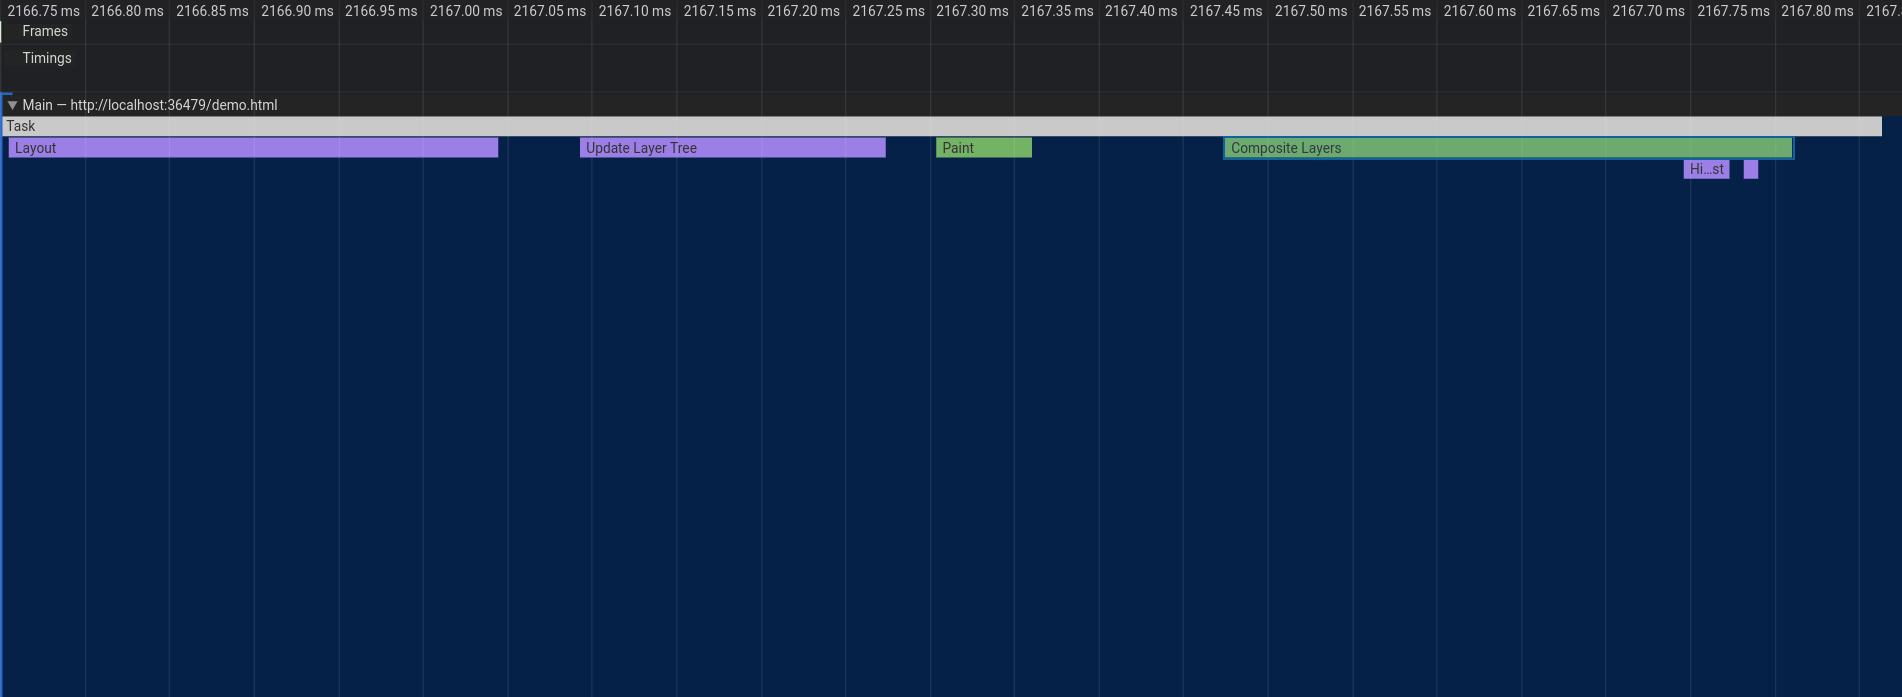
\includegraphics[width=0.8\columnwidth]{figures/experimental-setup/render-time-zoomed.png}
  \caption{An example of a Chrome profiler trace performed during the render of a component. The bar labeled ``composite layers'' signals our end time. Note that this falls just after a bar labeled ``paint'', signaling the paint event before the last composite event.}
  \label{fig:experimental-setup:render-time-end}
  \centering
\end{figure}

\section{First Paint \& First Contentful Paint}
In order to measure the first paint and first contentful paint, we construct a page that has the same content across all versions of the CC UI library. This means we construct one for the original Angular components, the Web Components version, and the various JS framework wrappers. We measure this metric by using the browser's built-in \code{performance} object. This object keeps track of both the FP and FCP metrics, allowing us to extract them.

\section{Number of Components}
The number of components is captured separately for the UI library as a whole and for the bundle described in Section~\ref{sec:experimental-setup:size}. Since the bundles described in Section~\ref{sec:experimental-setup:size} always contain three components, this number will always be three. The only exception is the CC UI library. For the CC UI library and the UI libraries captured as a whole, we gather the number of components by applying the process described in Section~\ref{sec:experimental-setup:gathering-components} to gather components, after which we count the number of them.
\chapter{Case Study}\label{chap:case-study}

In this chapter, we will be laying out the steps taken and the issues faced during the conversion from Angular components to Web Components. We will be splitting this section up into two subsections. The first subsection will consist of issues faced that were not specific to Angular or Angular elements, while the second subsection will contain just Angular-specific issues. Note that because of this split, the issues are no longer listed out in chronological order. For a chronological overview of the various issues and their relative complexities, see Table~\ref{tab:case-study:chronological-issues}. After the issue sections, we will discuss the various JS framework wrappers and how they were created. Lastly, we will be listing optimizations performed along with their effectiveness.

\begin{table}[h]
  \begin{tabularx}{\textwidth}{|l|X|l|}
    \toprule
    \textbf{Section}                            & \textbf{Section Name}              & \textbf{Relative Complexity} \\ \midrule
    \ref{sec:case-study:global-css}             & Global CSS                         & simple                       \\ \hline
    \ref{sec:case-study:compatibility}          & Compatibility                      & simple                       \\ \hline
    \ref{sec:case-study:tagname-renaming}       & Tagname renaming                   & simple                       \\ \hline
    \ref{sec:case-study:theming}                & Theming                            & simple                       \\ \hline
    \ref{sec:case-study:non-string-attributes}  & Non-string Attributes              & medium                       \\ \hline
    \ref{sec:case-study:complex-attributes}     & Complex Attributes                 & complex                      \\ \hline
    \ref{sec:case-study:ng-deep}                & ng-deep                            & simple                       \\ \hline
    \ref{sec:case-study:create-custom-element}  & createCustomElement                & simple                       \\ \hline
    \ref{sec:case-study:eventemitters}          & EventEmitters                      & simple                       \\ \hline
    \ref{sec:case-study:hierarchical-injectors} & Hierarchical Injectors             & hard                         \\ \hline
    \ref{sec:case-study:ng-on-init}             & ngOnInit                           & medium                       \\ \hline
    \ref{sec:case-study:casing}                 & Casing in attribute names          & simple                       \\ \hline
    \ref{sec:case-study:directives}             & Angular directives                 & simple                       \\ \hline
    \ref{sec:case-study:ng-content}             & <ng-content>                       & simple                       \\ \hline
    \ref{sec:case-study:attribute-order}        & Angular Attribute Order            & medium                       \\ \hline
    \ref{sec:case-study:bundling-imports}       & Bundling Angular Imports           & hard                         \\ \hline
    \ref{sec:case-study:ivy}                    & Angular Ivy                        & hard                         \\ \hline
    \ref{sec:case-study:searching-for-css}      & Reduce time searching for CSS      & simple                       \\ \hline
    \ref{sec:case-study:css-initial-load}       & Move CSS searching to initial load & simple                       \\
  \end{tabularx}
  \caption{Sections in chronological order along with their relative complexities}
  \label{tab:case-study:chronological-issues}
\end{table}

\section{Web Component Issues}~\label{sec:web-component-issues}
We will start off by describing any Web Component issues we faced. These are issues that are not at all related to the Angular framework and are likely to be faced in other similar projects.

\subsection{WC1: Global CSS}\label{sec:case-study:global-css}
\problemSolution{
  Angular components have a property called \code{encapsulation}\footurl{https://angular.io/guide/view-encapsulation\#view-encapsulation}. This property determines how CSS styles are applied to the component. It has three possible values:

  \begin{itemize}
    \item \emph{ShadowDom:} Global styles are not applied to the component. Only the component's own styles are applied to it.
    \item \emph{Emulated (default):} Global styles are applied to the component as well as its own styles. Other components' styles are not applied to it.
    \item \emph{None:} Global styles, a component's own styles, and other components' styles are applied to this component.
  \end{itemize}

  In the 30MHz codebase, the default value is used, meaning that both global and component-specific styles are applied to it. This is done by putting both of them in a global stylesheet. This stylesheet then has component-specific selectors added to it, making sure that styles are always scoped to a specific component. An example of this process can be seen in Listing~\ref{lst:case-study:component-css-source} and Listing~\ref{lst:case-study:component-css-compiled}.

  When converting the Angular components to Web Components, we ensure the components' contents are rendered within a ShadowRoot~\footurl{https://developer.mozilla.org/en-US/docs/Web/API/ShadowRoot}. This effectively separates the component from the rest of the DOM, thereby also removing the ability of the global stylesheet to be applied to it.

}{
  When a component is rendered, we find the global stylesheet on the page. We then copy it into a Constructable Stylesheet~\footurl{https://developers.google.com/web/updates/2019/02/constructable-stylesheets} if it has not already been copied. We then use the \code{adoptedStylesheets}~\footurl{https://developers.google.com/web/updates/2019/02/constructable-stylesheets\#using_constructed_stylesheets} property of a ShadowRoot to apply the global stylesheet in the component's own ShadowRoot as well. Because this Constructable Stylesheet is just a reference to a stylesheet that the browser re-uses, the performance impact of this process is minimal compared to copying the stylesheet's source code.

}

\begin{lstlisting}[language={JavaScript},caption={The source code for a component},label={lst:case-study:component-css-source}]
// my-component.html
<my-component></my-component>

// my-component.css
:host {
  color: red;
}
\end{lstlisting}

\begin{lstlisting}[language={JavaScript},caption={An example of compiled code for the component in Listing~\ref{lst:case-study:component-css-source}.},label={lst:case-study:component-css-compiled}]
// my-component.html
<my-component _ngcontent-uix-c290></my-component>

// my-component.css
[_ngcontent-uix-c290] {
  color: red;
}
\end{lstlisting}

\subsection{WC2: Compatibility}\label{sec:case-study:compatibility}
\problemSolution{
  While browser support for Web Components is relatively widespread as of this case study~\footurl{https://caniuse.com/?search=components}, it is not yet universal. Additionally, Safari has chosen not to implement support for so-called \emph{Customized Built-In Elements}\footurl{https://www.chromestatus.com/feature/4670146924773376}. This feature allows for extending built-in HTML elements, allowing developers to extend already-existing elements such as the \code{HTMLInputElement} and others. Since the 30MHz dashboard makes use of components that extend native elements (in the form of directives\footurl{https://angular.io/guide/attribute-directives}), we need this feature to make the CC UI library work.
}{
  We add so-called polyfills to the final JS bundle. These are files that add support for unsupported features by implementing them in different ways, using the built-in feature if there is already support for it. In particular we use the \ver{custom-elements}\footurl{https://www.npmjs.com/package/@ungap/custom-elements} and \ver{custom-elements-builtin}\footurl{https://www.npmjs.com/package/@ungap/custom-elements-builtin} polyfills.
}

\subsection{WC3: Tagname renaming}\label{sec:case-study:tagname-renaming}
\problemSolution{
  As per the Web Components specification, all Web Components are required to have a hyphen in their tag name~\footurl{https://html.spec.whatwg.org/multipage/custom-elements.html\#custom-elements-core-concepts}. Angular components, on the other hand, do not have this requirement. Because of this, there are some components in the 30MHz codebase without a hyphen in their name. In order to export them as Web Components, we need to come up with a tag name with a hyphen in it. In this case we decided to prefix every component with \code{cow-} (for example \code{<cow-checkbox>}). This renaming however leads to an issue with components that are being used inside other components. For example say the \code{DoubleCheckbox} component renders two checkboxes. Source code for such a component can be seen in Listing~\ref{lst:case-study:double-checkbox}. If such a component is rendered as a Web Component, it will attempt to render the \code{<checkbox>} HTML tag, not knowing that it has been renamed to \code{<cow-checkbox>}. The result is an empty component.
}{
  We run a pre-build script that replaces the names of components that will be used in the UI library with their prefixed variant. We make sure not to replace native HTML elements by matching the found HTML tags against a list of known native HTML elements.
}

\begin{lstlisting}[language={HTML},caption={The source code for a \code{DoubleCheckbox} component.},label={lst:case-study:double-checkbox}]
<checkbox id="checkbox-1"></checkbox>
<checkbox id="checkbox-2"></checkbox>
\end{lstlisting}

\subsection{WC4: Theming}\label{sec:case-study:theming}
\problemSolution{
  3rd party developers have expressed the wish to apply custom theming to their apps. In order to make this possible, we need to find a way to apply a single theme across all components on the page, regardless of ShadowRoots.
}{
  We make use of \emph{CSS Custom Properties}\footurl{https://developer.mozilla.org/en-US/docs/Web/CSS/Using_CSS_custom_properties}. These are effectively CSS variables that are defined for the whole document, including ShadowRoots. An example of the application of CSS Custom Properties can be seen in Listing~\ref{lst:case-study:custom-properties-js}. By changing the styles of the underlying Angular components to use CSS Custom Properties when available, we are able to provide theming. An example of this can be seen in Listing~\ref{lst:case-study:custom-properties-css}.
}

\begin{lstlisting}[language={JavaScript},caption={Applying CSS Custom Properties to the document},label={lst:case-study:custom-properties-js}]
function setPrimaryColorTheme(color: string) {
  document.documentElement.style.setProperty('color-primary', color);
}

setPrimaryColorTheme('red');
\end{lstlisting}

\begin{lstlisting}[language={CSS},caption={An example of a component making use of CSS Custom Properties},label={lst:case-study:custom-properties-css}]
my-component {
  /** 
    * Tries to use the --color-primary variable if available, 
    * falls back to blue when it is not defined.
    */
  background-color: var(--color-primary, blue);
}
\end{lstlisting}

\subsection{WC5: Non-string Attributes}\label{sec:case-study:non-string-attributes}
\problemSolution{
  As mentioned previously, it is not possible to pass non-string attributes to Web Components using just HTML\@. This presents an issue since some Angular components expect a non-string attribute to be passed. Examples include but are not limited to a boolean, a number, a JavaScript object with an \code{alignment} property, and a \code{Date} instance. While this is a problem that will be solved by our JS framework wrappers and particularly in Section~\ref{sec:case-study:complex-attributes}, the CC UI library should be at least usable by itself as well.
}{
  Because in this scenario, there is no access to JavaScript, we can not make use of any solutions to this problem that utilize the setting of attributes or properties through JavaScript. Instead, we need to use just HTML\@. The solution we came up with was to allow developers to optionally pass JSON to components by prefixing the attributes with \code{json-}. When this is done, the attribute value is parsed through \code{JSON.parse}, after which the corresponding property is set on the Web Component. This gives developers a way to pass most of the previously presented before. To allow developers to pass \code{Date} instances, we make it possible to pass strings, which we parse into Dates. While this is not a great workaround to have, especially since it only takes care of the \code{Date} class and not, for example, the \code{RegExp} class. The only way to fix this issue for all classes is to provide a method similar to Python \code{pickle}~\footurl{https://docs.python.org/3/library/pickle.html}, which, as mentioned on the documentation page, is not secure. We also feel like this problem is not prevalent enough in our case to warrant such a solution. Currently, all occurrences of classes as Angular component inputs have been taken care of.
}

\subsection{WC6: Complex Attributes}\label{sec:case-study:complex-attributes}
\problemApproachesImplementation{
  Continuing with the same problem, we now need to develop a way to solve the problem for even more situations, this time being able to use JavaScript since the solution will be implemented into the JS framework wrappers. Some of which include the passing of an object reference or an HTML element reference. This will never be possible through JSON since the reference needs to be preserved. Instead, we make use of JavaScript this time. Our goal is to allow a parent component written in the language of the JS framework to be able to pass its properties down to its child. This parent component is essentially just a passthrough component whose set of properties is identical. Its only purpose is to pass on these components and to provide a component native to the JS framework. Another thing to keep in mind is that we need all properties to be defined before the child component performs its first render. This issue is present simply because of the way the original Angular components are written, assuming that they will only receive attributes once and that they will never change.
}{
  There are a few approaches to solving this issue. These can be grouped into three categories.

  \begin{itemize}
    \item \emph{Parent \(\rightarrow\) child:} The parent node gets a reference to the child during the rendering process. Then the parent sets the properties on the child.
    \item \emph{Child \(\rightarrow\) parent:} The child gets a reference to the parent during the rendering process. It then requests its properties from the parent.
    \item \emph{Parent \(\rightarrow\) intermediary \(\rightarrow\) child, Child \(\rightarrow\) intermediary \(\rightarrow\) parent:} An intermediary takes the properties from the parent. The parent then provides the child with some way to find the intermediary, after which the child can get the properties from the intermediary upon rendering.
  \end{itemize}

  The first approach would be the easiest but this approach is not always possible. Many JS frameworks do not provide such low-level access to the to-be-rendered component. Instead, they often provide callbacks with a reference to the element after it has been connected to the DOM\@. Since the properties of our components need to be defined before they have even been rendered, this approach does not work for us.

  The second approach presents similar problems. While in some JS frameworks, it is possible to get a reference to the parent component, JS frameworks that use a virtual DOM such as React and Vue~\footurl{https://vuejs.org/} do not have a real parent component instance. Instead, the parent is just an abstract concept.

  This leaves us with the last approach—the creation of an intermediary object which holds the properties. The child is then given some way to get a reference to the intermediary (bypassing the problem of the second approach), after which it can get the to-be-applied properties from the intermediary. As long as we make sure the child has a way to find the intermediary access before it has been rendered to the DOM, we are able to fulfill the requirement of defining all properties before the first render.
}{
  Our implementation consists of several steps. We start by creating a class which we will call \emph{Intermediary}. This class has an instance manager attached to it, which we will call the \emph{IntermediaryManager}. Our JS framework wrapper code will be wrapping around the basic CC UI library. Since the CC UI library does not export the IntermediaryManager, we are unable to get a reference to it from our wrapper (aka the parent). In order to still get a reference to it, we want to store it globally. Because storing such properties on the \code{window} object can result in collisions and is unreliable, we will be storing it as a property of the defined Web Components. This means that we're able to access the \code{IntermediaryManager} property on the  \code{customElements.get('cow-checkbox')} object and get a reference to the IntermediaryManager from both the parent side and the child side.

  Now that we have taken care of this issue, we are able to start using it. We make the parent create an instance of an Intermediary. This Intermediary gets a simple string ID\@. We are then able to look up the ID in the IntermediaryManager and get the corresponding Intermediary. This ID is passed to the child, allowing it to look up this Intermediary.

  For passing the actual values, we make use of references. For each of the parent's properties, we pass the value to the Intermediary. The Intermediary then generates a unique string representing that value. If the Intermediary already knows the value, the same string is returned. Internally it maps this string to the value. We then pass this string to the child instead of passing the original complex value (which would not work). The child then receives the value and resolves it back to a complex value by consulting the Intermediary. Through this process, the child component is able to receive complex values from its parent through simple HTML string attributes.
}

\section{Angular Issues}
In this section, we will be describing any Angular related issues we faced. These are issues that were specific to Angular and are unlikely to be faced in similar projects when a different JS framework is being targeted.

\subsection{A1: ng-deep}\label{sec:case-study:ng-deep}
\problemSolution{
  Angular provides the \code{ng-deep} CSS selectors~\footurl{https://angular.io/guide/component-styles\#deprecated-deep--and-ng-deep}. Where regular CSS selectors stop at the ShadowDom boundary, meaning that a component will never be able to have a selector apply to the DOM of another component, the ng-deep selector does allow for this. It is an emulated and deprecated selector that does not work outside of Angular environments (including the Web Components environment). As such, we need to remove it.
}{
  The fix for this issue was fairly simple. Any instance of ng-deep had to be removed. While there has been some talk around browser support for a similar deep selector~\footurl{https://drafts.csswg.org/css-scoping/}, with both \code{::shadow} and \code{/deep/} making it into Chrome, they have since both been removed~\footurl{https://developers.google.com/web/updates/2017/10/remove-shadow-piercing}. As such, we had to come up with a workaround. Since the only way to effectively communicate from a component to child components is properties, we changed the code to use properties instead. An example of this change can be seen in Listing~\ref{lst:case-study:ng-deep-before} and Listing~\ref{lst:case-study:ng-deep-after}.
}

\begin{lstlisting}[language={JavaScript},caption={A component before the ng-deep change},label={lst:case-study:ng-deep-before}]
// parent-component.html
<child-component></child-component>

// parent-component.css
::ng-deep div {
  color: red;
}

// child-component.ts
@Component({
  ...
})
class ChildComponent {
  ...
}
\end{lstlisting}

\begin{lstlisting}[language={JavaScript},caption={A component after the ng-deep change},label={lst:case-study:ng-deep-after}]
// parent-component.html
<child-component red></child-component>

// parent-component.css
/**
 * ::ng-deep div {
 *  color: red;
 * }
*/

// child-component.ts
@Component({
  ...
})
class ChildComponent {
  @Input() red: boolean;

  constructor(private _elementRef: ElementRef) {
    if (this.red) {
      _elementRef.nativeElement.classList.add('red');
    }
  }
}

// child-component.css
:host[red] {
  color: red;
}

\end{lstlisting}

\subsection{A2: createCustomElement}\label{sec:case-study:create-custom-element}
\problemSolution{
  The main export of the Angular Elements library is the \code{createCustomElement} function~\footurl{https://angular.io/api/elements/createCustomElement}. This function takes an Angular component and turns it into a Web Component. It does this by extending an \code{HTMLElement} base class and applying all Angular component features on top of it. However, this function does not offer the ability to change the base class from an \code{HTMLElement} into anything else. As mentioned before, the 30MHz dashboard makes use of some elements that extend native elements. For example, the 30MHz input field extends the default HTML input field and only adds styling, preserving any built-in accessibility features provided by the browser. When converting this Angular component to a Web Component, we also wish to preserve these same features. This can be done by extending built-in HTML elements~\footurl{https://developer.mozilla.org/en-US/docs/Web/Web_Components/Using_custom_elements}. The \code{createCustomElement} function does not provide this option, causing us to be unable to create such an element. There is an open feature request for this option at the time of writing of this paper~\footurl{https://github.com/angular/angular/issues/19108}.
}{
  We have no choice but to implement this option ourselves. This means we have to copy the entire source code of the \code{createCustomElement} function, along with many of its dependencies, since very few of them are exported. After this, we change the function to allow us to pass such an option.
}

\subsection{A3: EventEmitters}\label{sec:case-study:eventemitters}
\problemSolution{
  Angular implements so-called \code{EventEmitters}~\footurl{https://angular.io/api/core/EventEmitter}. These are classes that are able to emit events, as well as being able to be listened to. When the \code{emit} function is called, the passed value is sent directly to those functions that added an event listener to it. Note that this behavior is different from regular event emitters, which emit a \code{CustomEvent}, which contains the actual value in the \code{detail} property. A lot of our Angular code relies on the value being directly emitted and it not being wrapped in a CustomEvent.

  When a component is converted to a Web Component, however, this emitted value is wrapped in a CustomEvent. Since the Angular code relies on this value being directly emitted, errors occur. In order to get around this issue, we need to make sure that internal code that listens to such EventEmitters receives the value itself, while external code (such as a 3rd party listening to a Web Component) receives the value wrapped in a CustomEvent.
}{
  We run a script that iterates over the source files, looking for any location where an event listener is being added to such an EventEmitter. Once we find one, we wrap the callback in an unwrapping function that strips away the CustomEvent and returns just the \code{code} value. An example of this change can be seen in Listing~\ref{lst:case-study:event-handler-change}.
}

\begin{lstlisting}[language={JavaScript},caption={A change made to an event listener. The definition of \code{unwrapEvent} can be seen in Listing~\ref{lst:case-study:event-handler-unwrap-event}},label={lst:case-study:event-handler-change}]
// before
(valueChanged)="myHandler($event)"

// after
(valueChanged)="myHandler(unwrapEvent($event))"
\end{lstlisting}

\begin{lstlisting}[language={JavaScript},caption={The \code{unwrapEvent} function},label={lst:case-study:event-handler-unwrap-event}]
function unwrapEvent(event) {
  if (event instanceof CustomEvent) {
    return event.detail;
  }
  return event;
}
\end{lstlisting}

\subsection{A4: Hierarchical Injectors}\label{sec:case-study:hierarchical-injectors}
\problemSolution{
  Angular makes use of a feature called \emph{Dependency Injection}~\footurl{https://angular.io/guide/dependency-injection}. This allows a parent module to provide its children with an instance of a particular dependency class. This class instance is shared among the module and its children. Generally, only modules provide their children with dependencies, where modules are simply collections of components that serve some common purpose. This dependency injection feature can also be leveraged to have a given component provide its own instance of a class only to its direct children. This means that every instance of that component gets its own separate instance of the dependency, which it then shares with its children, and not one that is shared across all components in the module. This is called \emph{Hierarchical Dependency Injection}\footurl{https://angular.io/guide/hierarchical-dependency-injection} and it is a feature that is utilized by 30MHz in some areas.

  Angular Elements does not support this feature intentionally~\footurl{https://github.com/angular/angular/issues/24824\#issuecomment-404399564}. Instead, it only supports the use case where modules provide their components with dependencies. The reason for this is that every component converted with Angular Elements is mounted to the DOM as its own root. It does not have a concept of a parent component and is unable to look up the injector of its parent. While the pattern of Hierarchical Dependency Injection is not recommended~\footurl{https://github.com/angular/angular/issues/24824\#issuecomment-404399564}, it is still a pattern used by 30MHz, and as such, we need to support it in order for the CC UI library to work.
}{
  Our goal in fixing this problem is to have a component injector inherit from its parent injector, which will facilitate Hierarchical Dependency Injection. To do this, we need to find the parent when the child is being rendered. After this, we can extract its injector, craft a new injector that combines the child and parent injector, and finally supply this new injector to the child. An example of this process can be found on StackBlitz~\footurl{https://stackblitz.com/edit/ngelements-issue-40104?file=src\%2Fapp\%2Fbar\%2Fbar.component.ts}.

  We first need to find the parent. This process is relatively straightforward. When the child is being rendered, we travel up the DOM tree until we find a node with specific properties that only Angular elements have. We then move on to the next stage of finding its injector.

  While the finding of a node's injector is straightforward in development mode since Angular exposes a \code{window.ng.getInjector} function, this process is a lot more complicated in production mode. To find it, we first need to find the component's hidden Angular properties. These can be found under the component's \code{\_\_ngContext\_\_} property. Depending on the environment, this can either be an object containing the so-called \code{tNode} and \code{lView} properties or an array that contains them at a magic offset. The \code{tNode} and \code{lView} are internal representations of a bunch of Angular-specific properties for the component.

  We are unable to access the original injector of the parent component since it is hidden in Angular-internal code. Instead, we need to use the \code{tNode} and \code{lView} to craft a new injector that will do the same thing as the original injector. However, in order to craft this new injector class instance, we need a reference to that same class. While a \code{Injector} class is exported from the Angular package, this is not actually the injector we want. Angular actually has two types of injectors, one of which is the previously mentioned \code{Injector} and the other is the so-called \code{NodeInjector}. This \code{NodeInjector} is only used internally, and it is the injector we want. To get a reference to it, we access the \code{injector} property of a fake component created by a \code{ComponentFactory}. Since the \code{ComponentFactory} is also not exported, we need to get a reference to it through the global injector. We now finally have a reference to the \code{NodeInjector} class, which allows us to re-create the parent's injector.

  We now merge this injector with the child injector. This is a relatively simple process. When a request for an injected value comes in, we first look for it in the child. If the child does not have it, we look at the parent injector.

  We now need to make sure Angular actually uses this injector we just created. To do so, we need to override the component's default element strategy (\code{NgElementStrategy}). This element strategy is a class provided by Angular that manages the connection between the DOM and the underlying Angular component. Since the \code{NgElementStrategy} class is also not exported by Angular, we need to find a reference to it somewhere. To do so, we create a fake component and read its \code{ngElementStrategy} property. We can now extend the class, replace the injector and provide it to the component. A complete code example of this process can be found in Listing~\ref{lst:appendix:hierarchical-injectors}.
}

\subsection{A5: ngOnInit}\label{sec:case-study:ng-on-init}
\problemSolution{
  Angular Elements does intentionally not guarantee the order in which attributes are set on an element (even initial attributes)~\footurl{https://github.com/angular/angular/issues/29050}. This means that attributes can be set on an element both before or after its main init hook (\code{ngOnInit}) is called. An example of this process can be seen in Listing~\ref{lst:case-study:ng-on-init}. While this is not a problem if attributes are only used to handle visual state, they can cause significant problems when used for component configuration. For example, if a component performs a fetch request to the server and takes a \code{URL} property that determines the target URL, it is essential that this property be set before the main hook runs. Quite a few components in the 30MHz codebase have a similar setup. As such, we need to guarantee that a component will always have the complete set of initial properties set before its main hook is called.
}{
  We know that, while the order of attribute setting is not guaranteed, we are guaranteed the fact that they will run sequentially. Since JavaScript is a single-threaded language and all attribute setting calls are synchronous, we know that all attributes will be set once the main thread is free again. For this, we use the global \code{window.requestAnimationFrame} JavaScript function. This function takes a callback and calls it when the main JavaScript thread is free to take on new work. We now firstly replace the component's \code{ngOnInit} function with an empty function, ensuring that when Angular calls it, the component's main hook is not actually run. We then call \code{window.requestAnimationFrame} and pass it the original \code{ngOnInit} function. Now we can guarantee that the \code{ngOnInit} function is called after all attributes have been set.
}

\begin{lstlisting}[language={JavaScript},caption={HTML source code and its Angular Elements equivalent},label={lst:case-study:ng-on-init}]
// HTML source file
<my-element foo="bar" bar="baz" />

// can be transformed into any of the following:
// 1
const element = document.createElement('my-element');
element.setAttribute('foo', 'bar');
element.setAttribute('bar', 'baz');
parent.appendChild(element);

// 2
const element = document.createElement('my-element');
parent.appendChild(element);
element.setAttribute('foo', 'bar');
element.setAttribute('bar', 'baz');

// 3
const element = document.createElement('my-element');
element.setAttribute('foo', 'bar');
parent.appendChild(element);
element.setAttribute('bar', 'baz');
  \end{lstlisting}

\subsection{A6: Casing in attribute names}\label{sec:case-study:casing}
\problemSolution{
  In the process of converting Angular components to Web Components, Angular Elements maps all input properties from camelCase casing to kebab-case. For example the input property \code{myInputProperty} is set through the \code{my-input-property} HTML attribute. The reason for this change is that HTML attributes are case-insensitive. To HTML \code{myInputProperty} is identical to \code{myinputproperty} and \code{MYINPUTPROPERTY}. While this is a good change to make and one that ensures that name collisions are less likely to happen, it does present some issues. Internal Angular elements still use the camelCase variant to set properties on their child components. Since the Web Component variants do not recognize the camelCase variant of the property anymore, they are ignored.
}{
  We solve this issue by making sure the Web Components also accept the camelCase variant. As HTML is case insensitive, there is no point in checking the casing of the passed attribute. Instead, we convert it to lowercase and compare it against the lowercase version of the original camelCase input property. In the previous example \code{myInputProperty}, \code{myinputproperty}, \code{MYINPUTPROPERTY}, and \code{my-input-property} would all refer to the input property \code{myInputProperty} on the Angular component.
}

\subsection{A7: Angular directives}\label{sec:case-study:directives}
\problemSolution{
  Angular has two types of elements that appear in the DOM\@. The first type is the Component, which looks for a given selector or tag name and replaces the original HTML element. For example an \code{AppRootComponent} with the selector \code{'app-root'} will look for an \code{<app-root>} HTML element and replace it with the Angular component instance. The second type is the Directive. Similarly, this looks for a selector, but instead of replacing the original HTML element, this simply mounts to it and runs its own code on it. An example of this would be a \code{Blink} directive that looks for the \code{'blink'} HTML class. When mounted, it periodically hides and un-hides the component.

  Angular Elements only supports the conversion of Components to Web Components, not the conversion of Directives. Since there are some elements in the 30MHz codebase that use Directives, we need to make sure that these are supported as well.
}{
  While this might sound like a challenging problem since these are entirely different elements, the fix for this issue is surprisingly easy. Under the hood, Angular stores the definition of a Component in the \code{\cmcrv{}cmp} property. This is also the property Angular Elements accesses to do the conversion from Angular components to Web Components. Similarly, the definition of Directives is stored in the \code{\cmcrv{}dir} property. By simply copying the value of the \code{\cmcrv{}dir} property to the \code{\cmcrv{}cmp} property, we are able to trick Angular Elements into thinking a directive is a component. Surprisingly, this works, and the directive works perfectly.
}

\subsection{A8: <ng-content>}\label{sec:case-study:ng-content}
\problemSolution{
  Angular uses the \code{<ng-content>} tag for so-called content projection. Content projection is the ability for a component to take a set of children, which it can then place anywhere in its DOM tree. This is effectively the same as the HTML \code{<slot>} tag~\footurl{https://developer.mozilla.org/en-US/docs/Web/HTML/Element/slot}. An example of content projection can be seen in Listing~\ref{lst:case-study:ng-content}. Content projection works fine in most scenarios, but sometimes it does not work. The child elements simply do not show up.
}{
  Our solution is once again quite simple; we take advantage of the fact that the \code{<ng-content>} and \code{<slot>} tag do the same thing and append a \code{<slot>} tag to every occurrence of an \code{<ng-content>} tag in the source code. This ensures that when the \code{<ng-content>} tag does not work, the \code{<slot>} tag takes over instead.
}


\begin{lstlisting}[language={HTML},caption={HTML source code and its Angular Elements equivalent},label={lst:case-study:ng-content}]
// parent-component.html
<child-component>
  <span id="my-span"></span>
</child-component>

// child-component.html
<div id="my-root">
  <ng-content></ng-content>
</div>

// Effective DOM tree
<parent-component>
  <child-component>
    <div id="my-root">
      <span id="my-span"></span>
    </div>
  </child-component>
</parent-component>
  \end{lstlisting}

\section{JS Framework Wrappers}
We wrote JS framework wrappers for a total of three JS frameworks. The first one is React. Since complex attributes for Web Components do not work natively in React, this wrapper was required in order to get the CC UI library to work in the first place. Since React provides good tooling when it comes to components and their properties, we felt it was a good idea to make use of this by providing typings for the CC UI library React wrapper. The second JS framework is Svelte. While Svelte works perfectly with Web Components out of the box, we created a wrapper to provide typings for the developers similar to React. The last JS framework is Angular itself. Angular also provides tooling, including built-in checking of component properties, which we felt we had to provide.

We also looked at different JS frameworks but found most of them to have little to no tooling for HTML elements. The UI libraries we looked at were Vue (v2 and v3)~\footurl{https://vuejs.org/}, Polymer~\footurl{https://www.polymer-project.org/}, lit-element~\footurl{https://lit-element.polymer-project.org/}, and wc-lib~\footurl{https://www.npmjs.com/package/wc-lib}.

In creating these wrappers, we started off by extracting the required component and type data from the components' source files. For example, the list of input properties, as well as their types and descriptions, need to be known. Similarly, all events emitted by the component, their types, and descriptions also need to be known. Finally, we also need to collect some metadata on the component itself, such as the name, tag name, and whether it has child elements. We extracted all this data by using the \emph{typescript} package~\footurl{https://www.npmjs.com/package/typescript}. This package allows for the parsing of TypeScript and JavaScript code. This code is turned into an abstract syntax tree (AST) with added type information, after which we are able to iterate through it. We extract all this data and turn it into a common format to be re-used by the various scripts that generate JS framework wrappers.

After collecting this data, we are able to generate the various JS frameworks. Generating wrappers was a reasonably smooth process for most JS frameworks. It consisted of iterating through the extracted component data and generating source files written in the language of the JS framework. These source files were then fed into a bundler and bundled into the wrappers. This process went smoothly for both the React and Svelte wrapper. During the process of creating an Angular wrapper on the other hand, we faced a few challenges. These challenges are described in detail below.

\subsection{A9: Angular Attribute Order}\label{sec:case-study:attribute-order}
\problemSolution{
  As previously described in Section~\ref{sec:case-study:ng-on-init}, the order in which Angular attributes are set is unknown. While we have fixed this issue for our Web Components in this section, this same issue presents itself again in the writing of an Angular wrapper. This time the problem is that components will be rendered before they have all of their input properties set. This leads to the apparent issue where the wrong contents are rendered.

  Another problem stems from our approach in Section~\ref{sec:case-study:complex-attributes}. We pass a unique ID to the child that is used to find the intermediary. When the child now receives an attribute that starts with the special reference prefix, it looks up the given reference by finding the intermediary and reading the attribute value. However, if the child receives such an attribute before having received the unique ID of the intermediary, it is unable to resolve the value. Since the order in which Angular attributes are passed is unknown, this situation arises very often.
}{
  We get around these issues by handling the appending to the DOM ourselves. Instead of having our Angular wrapper render the actual Web Components, we instead have them render a \emph{Renderer} component. This component is then passed the tag name of the Web Component. We are now able to precisely control when a component is appended to the DOM, as well as which attributes it gets and in what order. Since the \emph{Renderer} takes the place of the Web Component, it now receives all attributes. We wait until it has received the very last attribute before we decide to create the child component. After creating it, we apply all attributes the \emph{Renderer} has received to the child, after which we append it to the DOM\@. Since this process allows us such fine-grained control over the rendering cycle, we are able to render the Web Component without any issues.
}

\subsection{A10: Bundling Angular Imports}\label{sec:case-study:bundling-imports}
\problemSolution{
  Angular provides a few ways to build projects. Two of which are in use by us. The first option is to build a project as an application. This bundles everything into a combination of browser-specific bundles. These bundles can then smoothly be loaded by including them in the browser. This is the option we use for the Web Component library. The second option is to build a project as a library. Building a project as a library preserves all typing information and allows it to be used by another Angular project. Since we are building an Angular project, this is the option we need if we want to be able to provide typings to developers who use our Angular wrapper.

  However, we run into an issue after building. 30MHz uses the Font Awesome Pro~\footurl{https://fontawesome.com/pro} package for its icons. This is a licensed package that can only be downloaded when a valid key is presented. Since some of these icons are also used in the CC UI library, it needs to be bundled into the library to be able to work. Angular refuses to do this. They recommend using \code{peerDependencies}~\footurl{https://github.com/ng-packagr/ng-packagr/blob/v10.1.0/docs/dependencies.md} instead. While their reasoning for this is valid, it does not apply in our case. Since third-party developers are unable to install the Font Awesome Pro package without a license, they would run into an error when installing the package. Previously, Angular had the \code{embed} option, which allowed for the embedding of a given set of JS packages. This was eventually replaced with \code{bundledDependencies}~\footurl{https://github.com/ng-packagr/ng-packagr/issues/1106}, and a little while later, it was deprecated~\footurl{https://github.com/ng-packagr/ng-packagr/commit/0c52486}. This leaves us with no native option to bundle our dependency.
}{
  We fix this issue by programmatically changing the build artifacts Angular outputs. There are three types of build formats, the \code{FESM2015} (or flattened \code{ESM2015}), \code{ESM2015}, and \code{umd} formats. Bundling the Font Awesome Pro source code is fairly trivial for the \code{FESM2015} and \code{umd} formats since they are both single files. The \code{ESM2015} format is a bit different. It consists of a folder that is essentially a clone of the source code, with every TypeScript source file being replaced with a compiled JavaScript version and a \code{.summary.json} file. This \code{.summary.json} file functions similar to a \code{.d.ts} file, in that it provides type information of the file. In fixing our issue, we want to preserve this same folder structure. This means that we can not simply pass the entry point to a bundler and be done. On the other hand, we are also not able to feed every individual JavaScript file to the bundler. This would result in every separate file including its own copy of the Font Awesome Pro library, leading to a significant bundle size. Instead, we create a central folder in the \code{ESM2015} folder in which we store the Font Awesome Pro JavaScript bundle. This folder functions the same as a \ver{node\_modules} folder. We now replace every reference in the source files to point to this central location instead.
}

\problemSolution{
  We now run into another problem. When the library that was just built is used in an Angular project, the Angular compiler scans over all of its \code{.summary.json} files to build an AST with type information. It then finds the values that are exported, looks up their type values in the AST, and exports those that correspond to them. In performing this AST building process, the Angular compiler scans our included Font Awesome Pro folder for \code{.summary.json} files in order to extract definitions. Since those do not exist, an error is thrown.
}{
  The obvious approach to this problem is the following. We generate and bundle along the \code{.summary.json} files. This will provide Angular with the definitions it needs. The downside to this is that Angular will recursively perform this AST building process, meaning that it will first scan Font Awesome Pro, then its dependencies and their dependencies. All of these files would need to be included in the bundle simply to ensure the Angular compiler does not throw an error.

  Instead, the solution is to simply remove any reference to our bundled Font Awesome Pro library from the \code{.summary.json} files. Now that there is no longer a reference, the Angular compiler will simply skip over it. Since the Font Awesome Pro library is not exported, the Angular compiler never has to export any of its type information, meaning it does not actually need this data.
}

\subsection{A11: Angular Ivy}\label{sec:case-study:ivy}
\problemSolution{
  Angular has released a new version of its compiler called Ivy~\footurl{https://angular.io/guide/ivy}. This Ivy compiler is set to replace the previous View Engine compiler. Angular does not allow the use of Ivy for projects built as libraries for now~\footurl{https://angular.io/guide/ivy\#maintaining-library-compatibility} both because of compatibility reasons and because Ivy is not seen as stable enough as of the writing of this paper. This forces us to use the View Engine compiler instead. This compiler contains several bugs, one of which is causing the build to fail entirely in our case~\footurl{https://github.com/angular/angular/issues/25424}. This bug is marked as \ver{Fixed by Ivy}, however, we are unable to use Ivy.
}{
  The only other fix to this issue seems to be the disabling of AOT (or ahead-of-time compilation~\footurl{https://github.com/angular/angular/issues/25424\#issuecomment-465643237}. Unfortunately, the disabling of AOT introduces significant overhead during the loading of the built library, an issue that we have not been able to fix. As will be mentioned in the results section, this increases the load time of the Angular wrapper to an unacceptable level.
}

\section{Optimizations}
After finishing the CC UI library, we started looking for performance improvements. By looking through the Chrome profiler trace, we were able to find some easy performance improvements. These will be discussed in detail below.

\subsection{O1: Reduce time searching for CSS}\label{sec:case-study:searching-for-css}
We provide developers with a CSS file they should include in their final \code{index.html} file. This file contains the styles required to make the CC UI library work. We will be referring to this CSS file as the CC CSS file from now on.

As mentioned in Section~\ref{sec:case-study:global-css}, we find the CC CSS file on the page and copy it into every component instance. Since there can be many more stylesheets than just the CC CSS file, we need to scan every stylesheet and check whether it is the one. This searching process consists of the following steps.

\begin{itemize}
  \item Get a list of all stylesheets on the page, this includes both \code{<style>} tags and \code{<link rel="stylesheet">} tags.
  \item Iterate through every stylesheet.
  \item Iterate through every rule.
  \item Compare the current rule with a specific marker value that signifies the CC CSS file. If it matches, move on to the next step
  \item Add this stylesheet to the list of CC CSS files and move on to the next stylesheet.
\end{itemize}

While we did implement some caching, making sure this process only runs a single time, this process still has a significant performance impact. This performance impact scales linearly with the size of the stylesheet, meaning that a stylesheet with more rules takes longer to scan. It takes about 16ms to scan through a stylesheet of 1667 lines in order to find the marker rule on the machine mentioned in Section~\ref{sec:experimental-setup:machine-specs}. In addition to scaling with the size of the stylesheet, this number also scales with the number of stylesheets. Since it iterates through every available stylesheet, including a big stylesheet will vastly increase loading times.

We improve this process in two ways. The first step is to stop scanning after we find the marker simply. Instead of looking for other CC CSS files, we simply stop and return early. Since we know that there is only a single CC CSS file that applies to our Web Components, we can make this change. The performance impact of this change is hard to express in a single number since it largely depends on the stylesheets on the page, but this performance improvement saves about 1ms per 100 rules in stylesheets that are not the CC CSS file.

The second step is to ask the developers to help us in this process. We ask them to add a simple \code{cow} attribute to the \code{<style>} or \code{<link rel="stylesheet">} tag that contains the CC CSS file. Since the developer knows which file contains our supplied CSS file, they should easily add this attribute. At runtime, we check whether any stylesheet tags have a \code{cow} attribute. If there are, we can skip the entire process of finding the CC CSS file. Since this process was performed as the first component was rendered, this change saves about 16ms on the first component's render time.

\subsection{O2: Move CSS searching to initial load}\label{sec:case-study:css-initial-load}
While the above fixes provide excellent performance improvements, it may very well be possible that the developer does not add the \code{cow} tag, preventing our performance improvements from applying. The performance impact of the CSS search is still considerable, and the fact that it is run during the rendering of the first component significantly increases its render time. Since these render times tend to be around 16ms by themselves, a 16ms increase is enormous.

We remove this performance impact from the first render by moving it to the moment the CC UI library is initialized. To ensure we do not add any time to the initial load, we wait until the browser is idle by calling \code{window.requestIdleCallback}. This ensures that the process of finding CSS is performed while the browser is idle instead of it blocking an important operation such as component rendering.

\chapter{Results}\label{chap:results}
The metrics described in Chapter\ref{chap:design} have been collected for the created CC UI library. Using these metrics, we are able to compare the CC UI library to the original Angular components, the various JS framework wrappers, and various other UI libraries. In the following sections, the various metrics are broken down, and the results are compared between the various libraries.

\section{Render Time}
The render time metric allows us to evaluate the direct performance impact on users once the page has loaded. We first compare the CC UI library to the original Angular components and the other JS framework wrappers. This allows us to evaluate the performance impact added by the process of conversion to Web Components, as well as the performance impact added by the JS framework wrappers. After this, we compare the CC UI library to the UI libraries listed in Table~\ref{tab:design:ui-libraries}, allowing us to evaluate the performance of the CC UI library relative to UI libraries as a whole.

\subsection{Cow Components}
As mentioned in Chapter~\ref{chap:experimental-setup}, we have measured three basic components in particular that every UI library contains. These are the Button, Switch, and Input. We have measured the time needed to render 1 instance, 10 instances, and 100 instances of this component. The various render times for the cow-components UI libraries with these numbers of components can be seen in figures~\ref{fig:results:render-time-cow-1},~\ref{fig:results:render-time-cow-10}, and~\ref{fig:results:render-time-cow-100} respectively. We first take a look at the single-component render times. When we compare the performance of the CC UI library with the original Angular components, we find the CC UI library's median render time to be 81\% and 100\% higher for the Input and Switch components, respectively, with the mean render time for the Button being 41\% lower. Other than the Angular wrapper's Button (which is 100\% slower), the wrappers' render times are very similar. The React and Svelte Button rendering times are 6\% and 12\% lower, respectively, with both the Input and Switch render times being between 172\% and 190\% higher. From this, we can conclude that, although there is a full Angular root running for each component, the performance impact for a single component is minimal. Now taking a look at the render times for 10 and 100 components, we start to see some big differences. The Web Components version can still keep up with the original components when it comes to rendering 10 components, being 5\% faster, 144\% slower, and 111\% slower for the Button, Input, and Switch components, respectively. When rendering 100 components instances, however, it is eclipsed by the original components. Render times are 250\%, 393\%, and 265\% slower for the Button, Input, and Switch, respectively. It seems that the impact of creating a new Angular root for each component does become significant with many components.
Additionally, the render times for the various JS frameworks start to differ quite a lot. We see a trend of the React and Svelte wrapper growing further away from the Web Components version, with the average of the component render times increasing by 339\% for the React wrapper and 597\% for the Svelte wrapper. The Angular wrapper moves away even further, with the average of its component render times increasing by 735\%. It seems that the performance impact for rendering a relatively small amount of components is minimal, while it scales up relatively quickly with a greater number of components. The fact that picking a JS framework to develop in is especially interesting, potentially costing a difference of 150ms over Web Components or 50ms over a different framework.

\begin{figure}[h]
  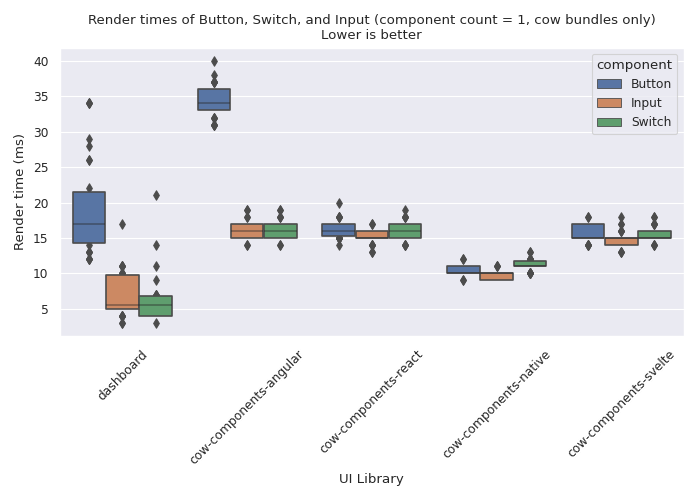
\includegraphics[width=\columnwidth]{plots/render-time-cow-1.png}
  \caption{Render times of a single Button, Switch, or Input component (CC UI only)}
  \label{fig:results:render-time-cow-1}
  \centering
\end{figure}

\begin{figure}[h]
  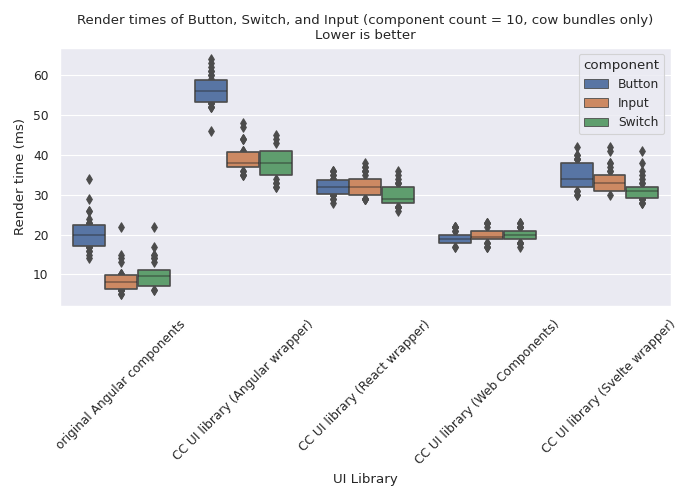
\includegraphics[width=\columnwidth]{plots/render-time-cow-10.png}
  \caption{Render times of ten Button, Switch, or Input components (CC UI only)}
  \label{fig:results:render-time-cow-10}
  \centering
\end{figure}

\begin{figure}[h]
  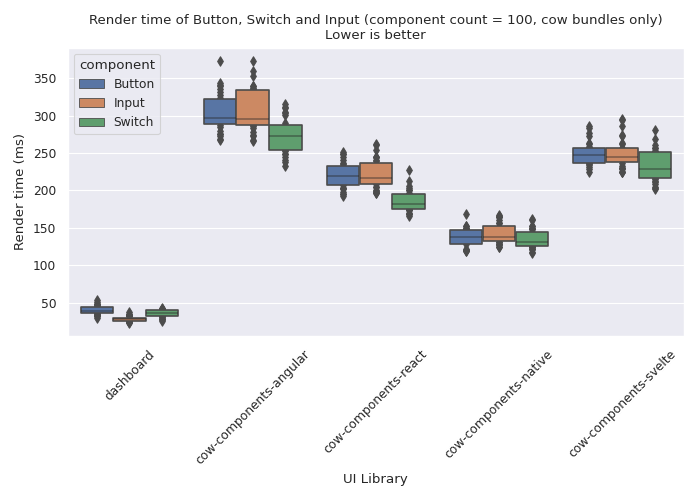
\includegraphics[width=\columnwidth]{plots/render-time-cow-100.png}
  \caption{Render times of one hundred Button, Switch, or Input components (CC UI only)}
  \label{fig:results:render-time-cow-100}
  \centering
\end{figure}

\subsection{UI Libraries}
We now compare the render times of the various UI libraries. Since the number of UI libraries we are comparing is very high (coming in at 29 total), showing them all in one figure makes for a very cluttered view. Instead, we compare a single component at a time. We have chosen to discuss the Button component in this section, however a complete overview can be found in Figures~\ref{fig:appendix:render-time-cow-1},~\ref{fig:appendix:render-time-cow-10}, and~\ref{fig:appendix:render-time-cow-100}. The render times of the Button component for the various UI libraries for 1, 10 and 100 components can be found in figures~\ref{fig:results:render-time-all-1},~\ref{fig:results:render-time-all-10}, and~\ref{fig:results:render-time-all-100} respectively.

\begin{figure}[h]
  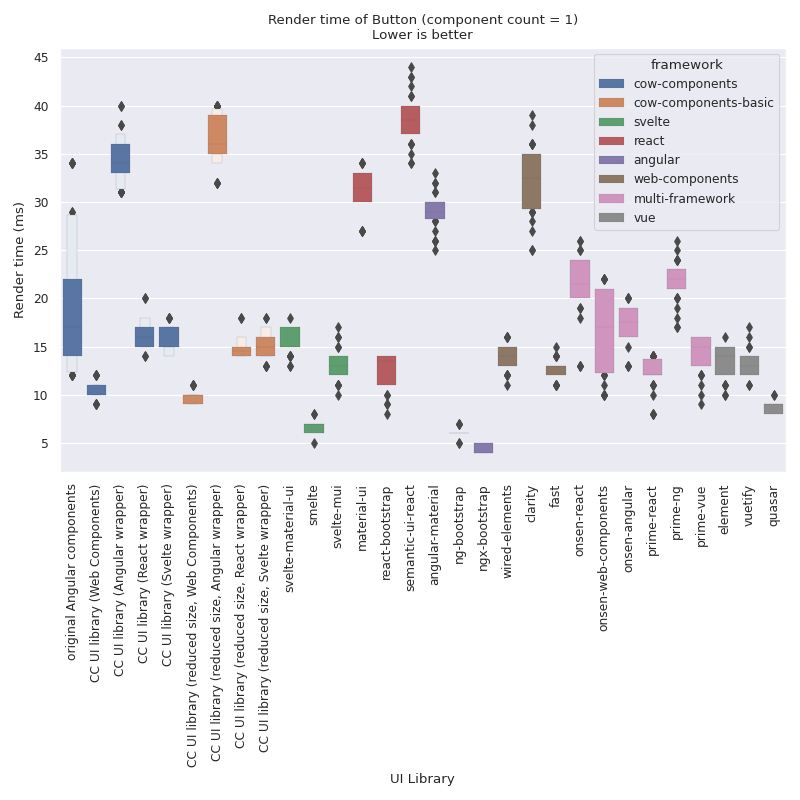
\includegraphics[width=\columnwidth]{plots/render-time-all-1-Button.png}
  \caption{Render times of a single Button. The reduced size CC UI library is the build of the library with less components, as described in Section~\ref{sec:experimental-setup:size}.}
  \label{fig:results:render-time-all-1}
  \centering
\end{figure}

\begin{figure}[h]
  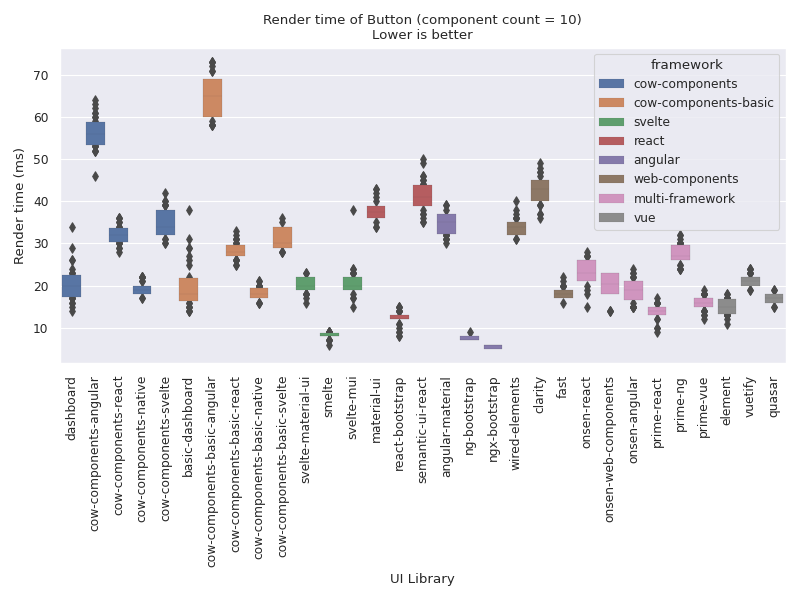
\includegraphics[width=\columnwidth]{plots/render-time-all-10-Button.png}
  \caption{Render times of 10 Buttons. The reduced size CC UI library is the build of the library with less components, as described in Section~\ref{sec:experimental-setup:size}.}
  \label{fig:results:render-time-all-10}
  \centering
\end{figure}

\begin{figure}[h]
  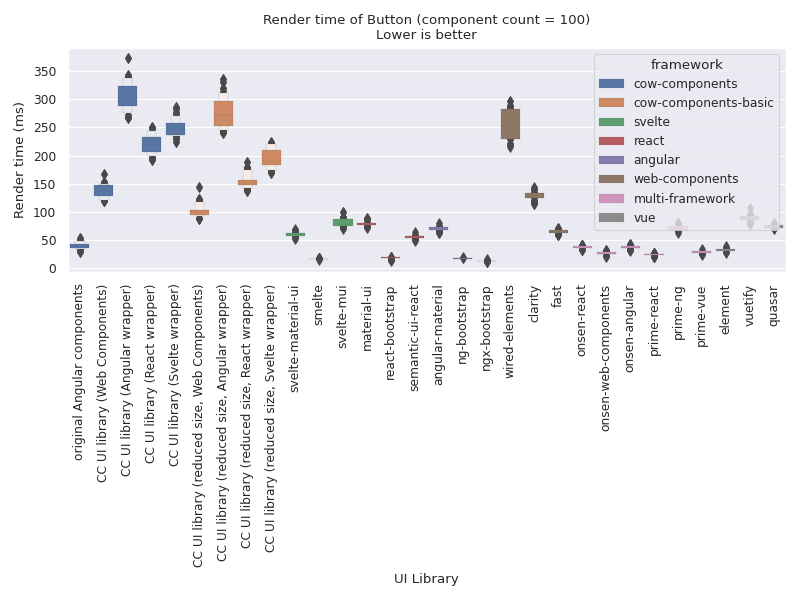
\includegraphics[width=\columnwidth]{plots/render-time-all-100-Button.png}
  \caption{Render times of 100 Buttons. The reduced size CC UI library is the build of the library with less components, as described in Section~\ref{sec:experimental-setup:size}.}
  \label{fig:results:render-time-all-100}
  \centering
\end{figure}

We, first of all, find that there are large differences in render times even within UI libraries that share the same framework. For example the render time for a button in \ver{react-bootstrap} is 57\% faster than \ver{material-ui} 64\% faster than \ver{semantic-ui-react}. In cases where this performance difference is relatively small, this has to do with the libraries themselves, but in a few cases, this has to do with the type of library. These libraries (\ver{react-bootstrap}, \ver{ng-bootstrap}, and \ver{ngx-bootstrap}) make use of a CSS framework, as laid out in section~\ref{sec:bg:ui-libraries}. As such, they are significantly faster and are essentially in a different category from the CC UI library, which is JS-based.

When we ignore these outliers, we can draw some conclusions on the average render times of the various frameworks. We first take a look at the single-component render times in Figure~\ref{fig:results:render-time-all-1}. We can see that Svelte UI libraries are generally swift, together having an average render time of 11.6ms. This falls in line with other performance benchmarks~\footurl{https://rawgit.com/krausest/js-framework-benchmark/master/webdriver-ts-results/table.html}. After this, Vue (12ms) and the UI libraries using Web Components (19,8ms) are the fastest. Interestingly, Web Components are slower than UI libraries using Svelte. Since Web Components are a native technology, one would be lead to believe that they would be faster. This might have something to do with how the authors of the UI libraries created their Web Components. It could be that their approach imposes a significant performance impact. The following frameworks when it comes to render time performance are Angular (29ms) and React (35ms). They are pretty close in performance, both being significantly slower than other frameworks. The previously mentioned performance benchmarks again support this.

We now apply our findings to the CC UI library JS framework wrappers. In our case, the Web Components version is the fastest simply because every other wrapper builds on top of this version. This means that it is impossible for another framework to be faster than it. We see this as well in the results, with the Web Components version coming in at 10ms. After that, the Svelte wrapper is the fastest, with a render time of 15ms. Interestingly, however, the React wrapper (16ms) is only slightly slower than the Svelte wrapper, while the Angular wrapper is significantly slower than both of them, coming in at 34ms. This is in contrast to what we just found, where both Angular and React were slow. It could be that the various internals of React that keep track of state and properties are slow. These are likely to be used a lot by regular React UI libraries, which need to handle their state entirely in React, while our React wrapper renders a component and passes it its properties once, making minimal use of methods exposed by React. In general, the CC UI library seems to be able to compete with the render times of other UI libraries, being faster than the vast majority of them.

\section{Load Time}
The load time metric allows us to evaluate the initial performance impact of the CC UI library. Again, we compare the various wrappers to each other as well as the original Angular components. As we elaborate on later, the Angular wrapper is significantly slower than any other UI library. For this reason, we split every figure into both a figure with and without the Angular wrapper. This should help show the scale of both this significant outlier while not reducing the scale's precision for other UI libraries.

\subsection{Cow Components}
The load time of the CC UI libraries can be seen in Figure~\ref{fig:results:load-time-cow-no-angular} (without the Angular wrapper) and Figure~\ref{fig:results:load-time-cow} (with the Angular wrapper). When we compare the load time of the CC UI library to the load time of the original 30MHz dashboard, we find that the CC UI library is significantly slower, coming in at 385ms compared to the 30MHz dashboard's 199ms. This is likely because the 30MHz dashboard has been optimized specifically for the initial load time. It loads the minimum amount of JavaScript needed to render the page. After this, other files are only loaded on an as-needed basis. The CC UI library, on the other hand, has to be contained in a single file. Splitting it up into multiple files and instructing third-party developers to have multiple JS bundles to make the CC UI library work would be a terrible developer experience. Concatenating the files into a single big bundle means all of the code has to be parsed and executed, slowing down execution by quite a lot.
Comparing the various wrappers to each other, we find the React and Svelte wrappers to have load times of 395ms and 434ms, respectively. This is only slightly slower than the CC UI library. The added load time is likely to be added by the JS frameworks themselves. Finally, we can see that the Angular wrapper is by far the slowest, with a load time of 4000ms. This is not entirely unexpected. As mentioned in Section~\ref{sec:case-study:ivy}, we had to disable AOT compilation for the Angular wrapper. This means all Angular compilation happens in the browser instead of during the compilation of the JS bundle. This is likely to be the reason why the Angular wrapper is so slow.

Taking a look at the reduced-size CC UI library, we find a loading time of 223ms for the CC UI library. This is only 12.6\% higher than the 30MHz dashboard. It appears that a significant portion of the loading was spent on these removed components. Further, the JS framework wrappers loading times are 588ms, 238m, and 277ms for the Angular, React, and Svelte wrappers, respectively. Again, the difference between the React and Svelte wrappers is minimal, with the Angular wrapper being significantly slower.

\begin{figure}[h]
  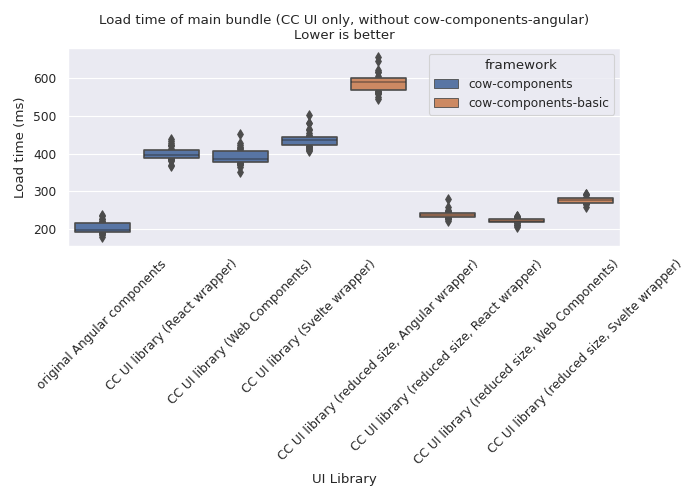
\includegraphics[width=\columnwidth]{plots/load-time-cow-no-angular.png}
  \caption{Load time of the main JS bundle (CC UI only, without Angular wrapper).}
  \label{fig:results:load-time-cow-no-angular}
  \centering
\end{figure}

\begin{figure}[h]
  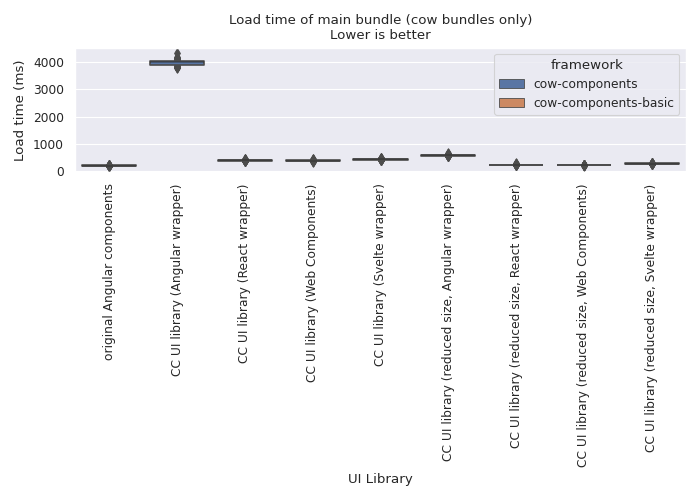
\includegraphics[width=\columnwidth]{plots/load-time-cow.png}
  \caption{Load time of the main JS bundle (CC UI only).}
  \label{fig:results:load-time-cow}
  \centering
\end{figure}

\subsection{UI Libraries}
The load times of other UI libraries can be seen in Figure~\ref{fig:results:load-time-all-no-angular} (without Angular wrapper) and Figure~\ref{fig:results:load-time-all} (with Angular wrapper). Other UI libraries largely differ in load time as well. Svelte UI libraries are by far the fastest, having an average load time of 2.64ms, followed closely by Web Components UI libraries at 11ms and React UI libraries with 22ms. After this, Vue UI libraries are the fastest, with a load time of 57ms. Finally, we have Angular, which with an average loading time of 106ms, is by far the slowest. Interestingly, we can see that the different distributions of multi-framework UI libraries follow this same pattern. For example the \ver{prime-ng} UI library is 329\% slower than the \ver{prime-react} UI library. Similarly, \ver{onsen-angular} is 167\% slower than \ver{onsen-react} and 308\% slower \ver{onsen-web-components}. This could also be one of the factors that are causing our Angular wrapper to be slower, although the lack of AOT compilation is still by far the most influential factor.

\begin{figure}[h]
  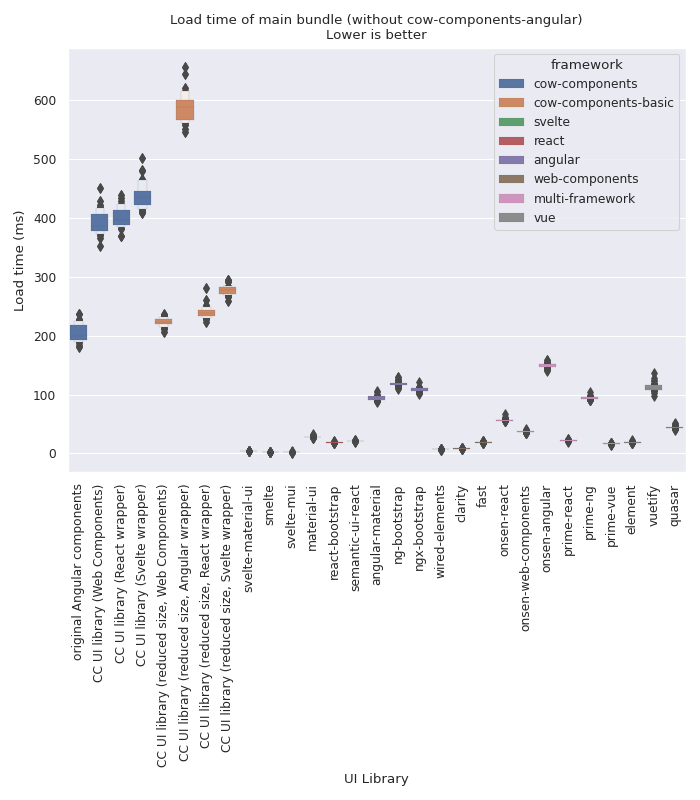
\includegraphics[width=\columnwidth]{plots/load-time-all-no-angular.png}
  \caption{Load time of the main JS bundle (without Angular wrapper).}
  \label{fig:results:load-time-all-no-angular}
  \centering
\end{figure}

\begin{figure}[h]
  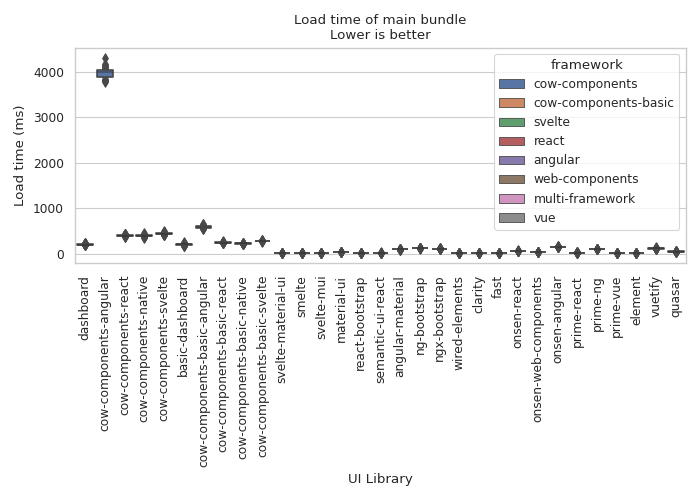
\includegraphics[width=\columnwidth]{plots/load-time-all.png}
  \caption{Load time of the main JS bundle.}
  \label{fig:results:load-time-all}
  \centering
\end{figure}

\section{Bundle Size}
Bundle size is a more abstract representation of the previous metric, allowing us to take a look at the impact of just the bundle size itself. This excludes any performance impact that can be attributed to poorly optimized code. This also allows us to look at what the performance impact of the Angular wrapper would be if there was no issue with the AOT compilation.

\begin{figure}[h]
  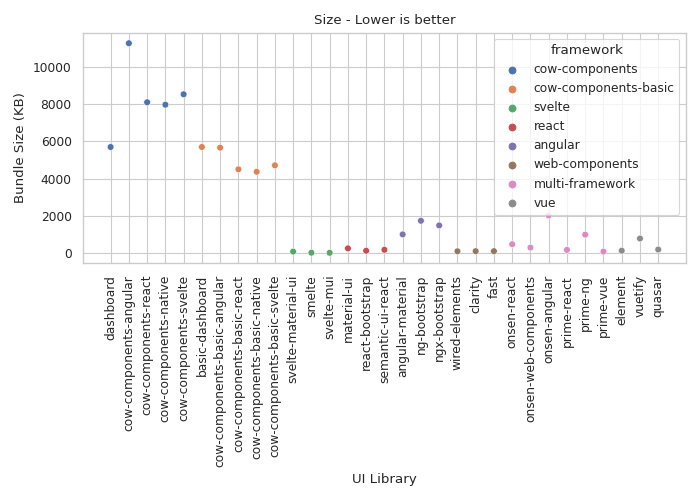
\includegraphics[width=\columnwidth]{plots/size.png}
  \caption{Size of the main JS bundle.}
  \label{fig:results:size}
  \centering
\end{figure}


The various bundle sizes can be found in Figure~\ref{fig:results:size}. We can first of all see that the bundle sizes correlate strongly with the load times. From this, we can conclude that they are an excellent representation of the load time metric. We find sizes average sizes of 57KB, 120KB, 204KB, and 385KB for Svelte, Web Component, React, and Vue UI libraries, respectively. As expected, Angular is by far the biggest, with a size of 1422KB. This same trend is also visible in our various wrappers. The Angular wrapper is by far the biggest, with a size of 11,251KB. With the strong correlation between load time and bundle size, we can conclude that a large part of the Angular wrapper's slow load time can be attributed to the large bundle size.

\section{Page Load Time}
The page load time metric should give us an idea of the real-world loading time of the CC UI library. As described in Chapter~\ref{chap:experimental-setup}, we replicated a page containing all components in the various distributions of the CC UI library. This means that all versions are rendering essentially the same page but in their own framework.

The resulting page load times can be found in Figure~\ref{fig:results:first-paint}. We have included both the \ver{First Paint} and \ver{First Contentful Paint} metrics, which are entirely the same for all the wrappers, only differing for the 30MHz dashboard. We find a first paint of 194ms and a first contentful paint of 233ms for the 30MHz dashboard. The Web Components version of the CC UI library has a first paint (and first contentful paint) of 25ms. This is 87\% faster than the 30MHz dashboard. This is likely because the dashboard also needs to run background tasks. These are tasks such as checking whether a user has logged in and fetching data. The CC UI library, on the other hand, has been stripped of this unneeded functionality. Apart from this, we can see a familiar trend of React and Svelte being slightly slower than the original, with first paint times of 618ms and 616ms, respectively. Finally, we find the Angular wrapper to have a first paint time of 2029ms.

\begin{figure}[h]
  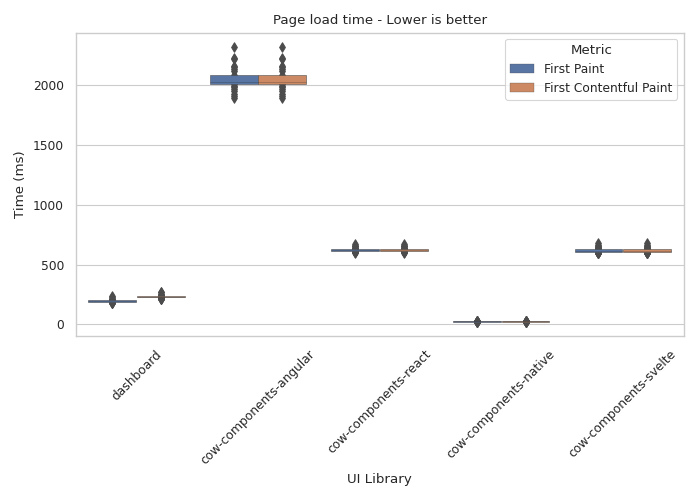
\includegraphics[width=\columnwidth]{plots/first-contentful-paint.png}
  \caption{First paint metrics for the various demo pages.}
  \label{fig:results:first-paint}
  \centering
\end{figure}

\section{Quality of Web Components}
In this section, we take a look at the quality of the Web Components in the CC UI library. Note that we essentially measure the quality of the original Angular components. This means that the conclusions drawn in this section only apply to the 30MHz codebase and will not be the same for other source codebases.

\begin{figure}[h]
  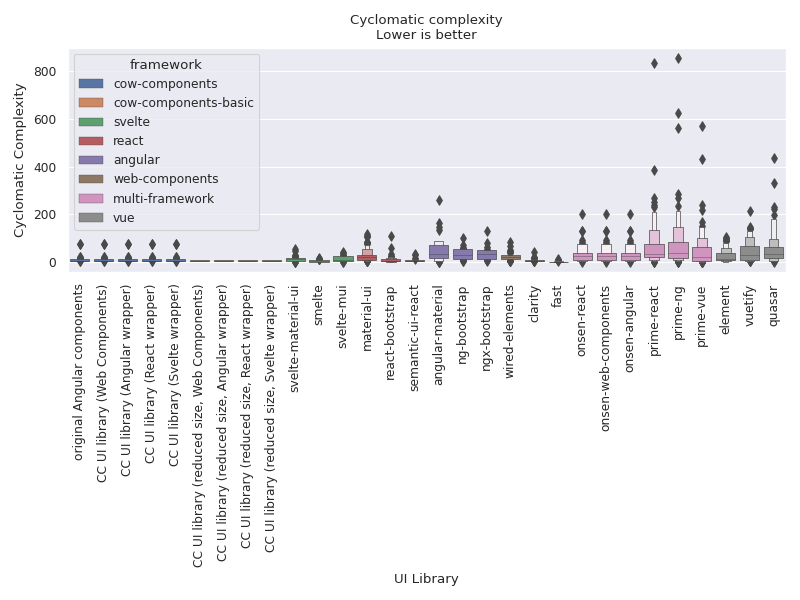
\includegraphics[width=\columnwidth]{plots/cyclomatic-complexity.png}
  \caption{Cyclomatic complexity of the various UI libraries.}
  \label{fig:results:cyclomatic-complexity}
  \centering
\end{figure}

\textbf{Cyclomatic complexity:} The cyclomatic complexities of the various UI libraries can be seen in Figure~\ref{fig:results:cyclomatic-complexity}. The cyclomatic complexity of the CC UI library is has a median value of 2 and a mean value of 10.4. The average cyclomatic complexity of the medians of all UI libraries is 17.5. Multi-framework UI libraries, in particular, have a very high cyclomatic complexity. The median cyclomatic complexity for all \ver{onsen}-based UI libraries is 22, while the cyclomatic complexities for \ver{prime-react}, \ver{prime-ng}, and \ver{prime-vue} are 31.5, 36, and 18 respectively. This makes sense since these libraries often try to share the source code between the various frameworks as much as possible, leading to many imports.

\begin{figure}[h]
  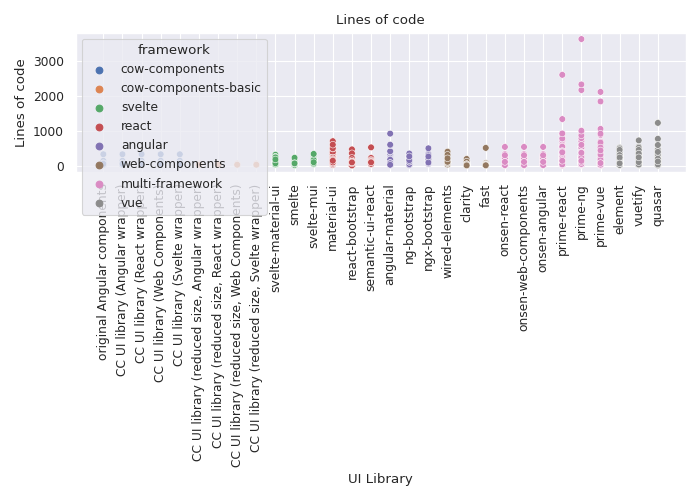
\includegraphics[width=\columnwidth]{plots/lines-of-code.png}
  \caption{Lines of code of the various UI libraries.}
  \label{fig:results:lines-of-code}
  \centering
\end{figure}

\textbf{Lines of code:} The amounts of lines of code can be seen in figure~\ref{fig:results:lines-of-code}. Again we see the same trend of the CC UI library being relatively low in complexity (and as such lines of code), with the median lines of code being 26. The average of the medians of all UI libraries is 108.75.

\begin{figure}[h]
  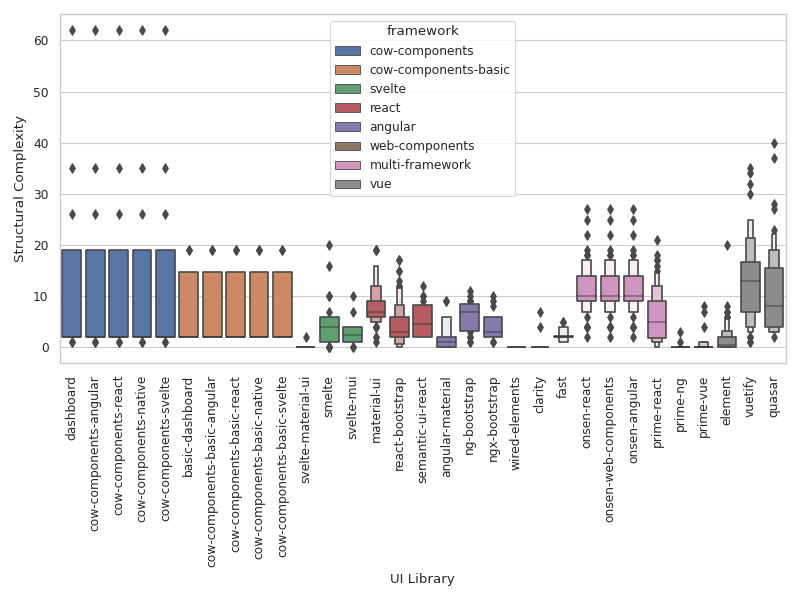
\includegraphics[width=\columnwidth]{plots/structural-complexity.png}
  \caption{Structural complexity of the various UI libraries.}
  \label{fig:results:structural-complexity}
  \centering
\end{figure}

\textbf{Structural complexity:} The structural complexities can be seen in figure~\ref{fig:results:structural-complexity}. This time there is a large variation in the structural complexity of CC UI library components, with the median being 2 and the average being 12.6. This outlier is likely to be the Chart component, which is by far the biggest component. The average of the other UI libraries' median structural complexity is 4.2. This suggests that the median structural complexity of the CC UI library is relatively low, which is good.

\begin{figure}[h]
  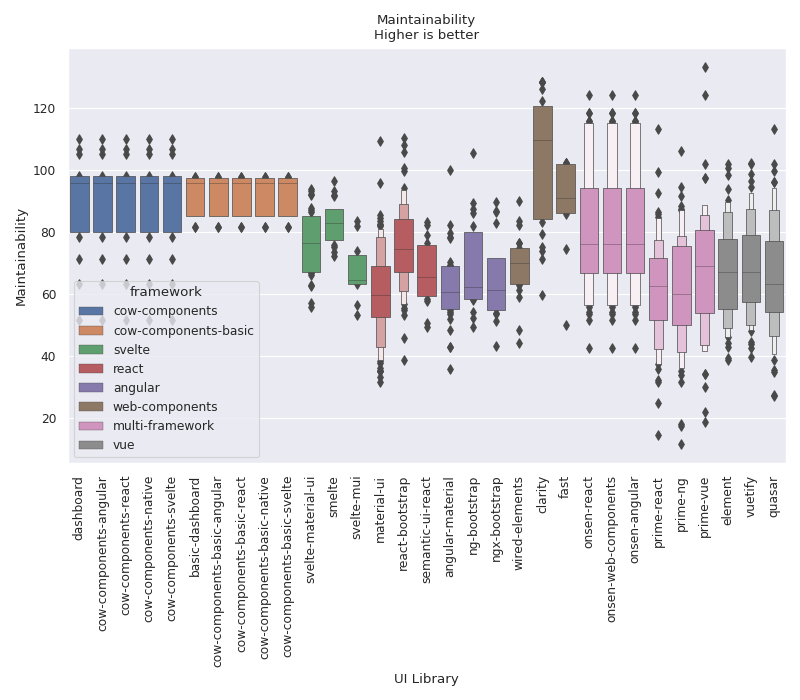
\includegraphics[width=\columnwidth]{plots/maintainability.png}
  \caption{Maintainability of the various UI libraries.}
  \label{fig:results:maintainabilty}
  \centering
\end{figure}

\textbf{Maintainability:} The maintainabilities can be seen in figure~\ref{fig:results:maintainabilty}. The median maintainability of the CC UI library is 96, with the average median maintainability of the UI libraries being 71. Higher maintainability is better, meaning the CC UI library scores quite well in this metric. All together, we can conclude that the quality of the CC UI library components (and as such, the Angular components they are based on) is quite high.

\section{Time spent on the project}\label{sec:results:time-spent}
While the technical results of this project are important, we also decided to take a look at the business side of this project. An important factor here would be the amount of effort required to complete this project. In total, this project took five months of fulltime-equivalent (FTE) to complete. An estimation would be that about one month was spent on Web Component related issues, three months on Angular related issues and one month on creating JS framework wrappers, and one month on other tasks such as creating a build pipeline and package distributions. Note that the time taken is entirely separate from the number of components in the resulting UI library, meaning an added component would not increase the time taken at all. Depending on the time required to build the UI library from scratch combined with the time taken to maintain the UI library and adding new components, this project could very well be worth it. \todo{}
\chapter{Threats to Validity}\label{chap:threats-to-validity}

In this chapter, we will be covering threats to the validity of this study. Firstly we will discuss the internal validity, after which we will discuss the external validity of the study.

\section{Internal Validity}
Possible internal threats to validity would be the measurement of our metrics being influenced by external factors. As described in Section~\ref{sec:experimental-setup:load-time} we explicitly remove the factor of network speed from our benchmarks. This leaves only the factor of available system resources as a possible variable. In order to eliminate this factor, we took several steps. We first ensured a clean testing environment by shutting down all unneeded background processes on the test machine. This should vastly reduce the amount of fluctuation in available system resources. Secondly, we ensured that only a single test is running at a time. This means every test has the entire computer to itself (in practice, likely a single core) and does not compete with other tests for system resources. Lastly, we apply all the steps described in Section~\ref{sec:experimental-setup:time-sensitive-metrics} which includes randomizing the order in which the tests are run and increasing the number of tests to \numMeasures{} measurements per test. This should ensure that any possible fluctuations are smoothed out and shared across all tests.

\section{External Validity}
A large number of problems in this case study faced applied to Web Components in general, as shown in Section~\ref{sec:web-component-issues}. Still, a significant share of the problems is related to Angular, more specifically Angular 10. Likewise, a significant part of them is specific to the 30MHz codebase. Given a different codebase or a different Angular version, different problems might be faced in the process of converting Angular components to Web Components. While the issues might differ from framework to framework or even from Angular version to Angular version, the results should be generalizable to other frameworks and Angular versions. Bugs we encountered are likely to be fixed, and performance is likely to only improve in future Angular versions, as has been the case with the Angular Ivy compiler~\footurl{https://angular.io/guide/ivy}. Additionally, a significant amount of the faced problems apply to Web Components in general, as shown in Section~\ref{sec:web-component-issues}. For this reason, we believe that the feasibility of the applied process will at worst stay the same and at best improve for other Angular versions or JS frameworks.
Further, while the specific UI library we created is dependent mainly on the 30MHz codebase and its specific architecture and contents, we make sure to compare the created CC UI libraries with the original 30MHz codebase itself, ensuring all results are relative to the original. This should ensure we answer the research question for a generalized case. If we were to compare the CC UI library solely to other UI libraries, the answer to the research question would only apply to the case of 30MHz. \todo{}
\chapter{Discussion}\label{chap:discussion}

The results described in Chapter~\ref{chap:results} show that the creation of a UI library from an existing codebase is very well possible in an Angular application. Render times are only slightly higher, remaining competitive with various other UI libraries. One negative aspect seems to be that the render times increase quite quickly with a higher number of components. Further, load times are not significantly higher in all cases except the Angular wrapper. This all should result in a good user experience across the board, being slightly slower than the original components but providing access to them in most popular JS frameworks. We can say that the answer to SRQ1 is that it is definitely technically feasible to convert Angular components to Web Components.

While the technical results of this project are important, we also evaluated the business side of this project through SRQ2. We find the time spent to be five months of FTE\@. We also took a look at the degree in which this project interferes with the original codebase and its developers' workflows. In questioning the three front-end developers at 30MHz, we found that on average they rated the impact of changes to the main codebase as a 2.6 on a scale from 0 (no impact at all) to 10 (significant impact). For a process that interlocks with the main codebase so heavily, this is a very low number, leading us to believe that the impact was small. Additionally, there are some new factors that developers have to keep in mind while developing new components. An example of this is the need for better documentation for components in order to ensure the automatically generated documentation is correct. Another example would be the need to add a new UI component to the array containing all components that are to be included in the UI library. On average the developers rated the impact of these changes to be a 2, signaling that the every day impact is not very large. Lastly, we asked developers how often their workflow was blocked by the existence of this project. All of them indicate they have not been blocked once, meaning this project was executed completely in parallel and without blocking other developers' workflow. These results suggest that the answer to SRQ2 is that the business viability of the conversion of Angular components to a UI library is quite high as well, leading to minimal impact on current developers and their workflow, while requiring relatively little time. Especially in a situation where there are a large number of UI components, the time spent on this project is significantly smaller than the time spent recreating them.

All in all we can conclude that the answer to RQ1 is that the process of converting Angular components to a Web Component UI library is quite feasible. We hope this case study convinces businesses who are considering this process to take the steps we have taken over the creation of an entirely new UI library. In addition to being used in the manner we described, that is the creation of a UI library for 3rd parties, this process could also be applied to components that are internal to a business. With the ever increasing amount of platforms with which users are able to interact (desktops, phones, tablets, televisions, smart fridges), the number of platforms for which businesses need to develop an application also increases. Since most of these platforms require different software stacks, Web Components could provide a basis off of which to generate components for other platforms. For example the main large web app can be built in Angular, with another small internal web app being built in React (using the React wrapper), another internal web app built in Vue, and the mobile apps built using React Native~\footurl{https://reactnative.dev/} or Apache Cordova~\footurl{https://cordova.apache.org/}.

What the results of these study do not tell us is the viability of converting components from any other JS framework to Web Components. In this case study we specifically targeted Angular, which provides the simple Angular Elements tool~\footurl{https://angular.io/guide/elements}. Other JS frameworks might not have such tools available, which might make this process less straightforward. However, we believe that the process of converting components from any other popular JS framework to Web Components may very well be significantly easier than from Angular components. A large number of the issues we faced were Angular related, as described in Section~\ref{sec:case-study:ng-deep}. Those issues were also by far the hardest to solve. Most of these issues would not appear when using other JS frameworks.

As mentioned, this case study only allows us to draw conclusions of the viability of converting \textbf{Angular} components to Web Components. As such, we think a good starting point for further research is research into this same process for other JS frameworks. If this process is proven to be viable for other JS frameworks as well, businesses would be able to convert their components to Web Components regardless of their original JS framework, allowing for this process to be far more widely used. \todo{}
\chapter{Conclusion}\label{chap:conclusion}

In this case study, the feasibility of converting a set of Angular components to Web Components was evaluated. Chapter~\ref{chap:case-study} describes the various issues we faced during this project, eventually showing that it is possible to convert a set of Angular components to Web Components. In Chapter~\ref{chap:results} we evaluate the end resulting Web Components, comparing them to both the original Angular components they were created from and various other UI libraries. We find that the newly created Web Components are only slightly slower in rendering and take only about twice as much time to load. The resulting components hold up very well compared to other UI libraries, initially being faster than quite a few of them but becoming relatively slower as the number of rendered components increases. This means that although the Web Components library was converted from Angular components, it can compete quite well with other UI libraries that were written from scratch. This confirms the technical feasibility of converting Angular components to Web Components.

Further, when looking at the business side in Section~\ref{sec:results:time-spent} and Chapter~\ref{chap:discussion}, we find that the impact on the existing codebase and other developers is minimal. We also find the time spent on this conversion to be definitely worth it depending on the time required to build the UI library from scratch combined with the time taken to maintain the UI library and adding new components. This indicates that this conversion is a worthwhile investment, leading to freedom from maintaining two sets of components and the ability to easily add a new component to the Web Components library without issues. It should be noted that these results are not based on sufficient data to draw definitive conclusions. Instead, we indicate that these were our results and leave definitive proof for future work.

One shortcoming of this thesis is that we were only able to evaluate the effectiveness of converting \textbf{Angular} components to Web Components. Not the conversion of components from any JS framework to Web Components. We theorize that this process should be just as feasible, with other frameworks likely taking significantly less time to convert than Angular. As such, we believe further research into the conversion of components from other JS frameworks to Web Components would be very beneficial, eventually leading to a situation where we can conclude that components from all JS frameworks can be converted to Web Components, eventually making them re-usable across all JS frameworks. \todo{}
\clearpage
\appendix
\chapter*{Appendix}

\section{Code for creating a Hierarchical Injector in an Angular Elements component}

\begin{lstlisting}[language={JavaScript},caption={The code for creating a Hierarchical Injector in an Angular Elements component},label={lst:appendix:hierarchical-injectors}]
	// This injector is provided by Angular to the root module
	var rootInjector = ...;
	
	// Create a fake injector
	const _MOCK_INJECTOR = {
		get() {
			return {
				run() {},
				resolveComponentFactory() {
					return {
						inputs: [],
					};
				},
			};
		},
	};
	
	// Extract defualt NgElementStrategy
	function getDefaultNgElementStrategy() {
		const customElement = createCustomElement(EmptyAngularComponent, {
			injector: _MOCK_INJECTOR,
		});
		const proto = customElement.prototype;
		const strategyInstance = proto.ngElementStrategy;
		return strategyInstance.constructor;
	
	}
	
	// Get the NodeInjector class
	function getNgInjectorClass(rootInjector) {
		const componentFactory = rootInjector.get(ComponentFactoryResolver).resolveComponentFactory(EmptyAngularComponent);
		const componentInstance = componentFactory.create(rootInjector, []);
		return componentInstance.injector.constructor
	}
	
	// Get given HTML element's nodeinjector
	function getNodeInjector(rootInjector, host) {
		const hostContext = host.__ngContext__;
		const lView = hostContext.lView;
		const tNode = lView[1].data[hostContext.nodeIndex];
		const NodeInjectorClass = getNgInjectorClass(rootInjector);
		return new NodeInjectorClass(tNode, lView);
	}
	
	// Create a custom NgElementStrategy
	class CustomNgElementStrategy extends getDefaultNgElementStrategy() {
		originalInjector = this.injector;
	
		connect(element): void {
			if (this.injector === this.originalInjector) {
				const localRoot = element.getRootNode();
				const host = localRoot.host;
				const nodeInjector = getNodeInjector(rootInjector, host);
	
				this.injector = Injector.create({
					providers: [],
					parent: nodeInjector,
				});
	
				return this._connectSuperWithDelayedInit(element);
			}
	
			return super.connect(element);
		}
	}
	
	// Create a custom NgElementStrategyFactory that creates
	// instances of our custom NgElementStrategy
	class CustomNgElementStrategyFactory {
		constructor(
			private _StrategyConstructor,
			component,
			injector,
		) {
			this.componentFactory = injector
				.get(ComponentFactoryResolver)
				.resolveComponentFactory(component);
		}
	
		create(injector) {
			return new this._StrategyConstructor(this.componentFactory, injector);
		}
	}
	
	// Provide the CustomNgElementStrategyFactory to the createCustomElement
	// function and create a new Web Component
	const WebComponent = createCustomElement(AngularComponent, {
		injector: rootInjector,
		strategyFactory: new CustomNgElementStrategyFactory(
			CustomNgElementStrategy,
			AngularComponent,
			rootInjector
		)
	})
		\end{lstlisting}

\clearpage
\bibliographystyle{lib/PhDbiblio-url2}
\renewcommand{\bibname}{References}
\bibliography{bib/references}

\end{document}
